% This is samplepaper.tex, a sample chapter demonstrating the
% LLNCS macro package for Springer Computer Science proceedings;
% Version 2.21 of 2022/01/12
%
\documentclass[runningheads]{llncs}
%

\usepackage{geometry}
\geometry{
  a4paper,         % or letterpaper
  textwidth=12.6cm,  % llncs has 12.2cm
  textheight=21cm, % llncs has 19.3cm
  heightrounded,   % integer number of lines
  hratio=1:1,      % horizontally centered
  vratio=2:3,      % not vertically centered
}
% \renewcommand\floatpagefraction{.3}
\usepackage{tabularx}
\usepackage{scrextend}
\changefontsizes{9.5pt}
\newcolumntype{Y}{>{\centering\arraybackslash}X}
\setlength{\abovecaptionskip}{1ex}
\setlength{\belowcaptionskip}{1ex}
\setlength{\floatsep}{1ex}
\setlength{\textfloatsep}{1ex}
\usepackage{setspace}
\usepackage{titlesec}
\titlespacing\section{0pt}{10pt plus 4pt minus 2pt}{4pt plus 2pt minus 2pt}
\titlespacing\subsection{0pt}{10pt plus 4pt minus 2pt}{4pt plus 2pt minus 2pt}
\titlespacing\subsubsection{0pt}{4pt plus 4pt minus 2pt}{4pt plus 2pt minus 2pt}





\usepackage[T1]{fontenc}
\usepackage{comment}

% T1 fonts will be used to generate the final print and online PDFs,
% so please use T1 fonts in your manuscript whenever possible.
% Other font encondings may result in incorrect characters.
%
\usepackage{graphicx}
% Used for displaying a sample figure. If possible, figure files should
% be included in EPS format.
%
% If you use the hyperref package, please uncomment the following two lines
% to display URLs in blue roman font according to Springer's eBook style:
%\usepackage{color}
%\renewcommand\UrlFont{\color{blue}\rmfamily}
%
% \documentclass[twoside]{article}
\usepackage{amsfonts,amssymb,amsbsy,textcomp,marvosym,picins,amsmath,caption,threeparttable,amsthm,subfigure,float,lastpage,lscape}
\usepackage{eurosym,mathrsfs,fancyhdr,CJK,multicol,graphics,indentfirst,color,bm,upgreek,booktabs,graphicx,multirow,warpcol}
\usepackage{amsmath}
\usepackage{algorithm}
\usepackage{algpseudocode}
\usepackage{amsfonts}
\usepackage{epstopdf}
\usepackage{graphicx}
\usepackage{subfiles} 
\usepackage{hyperref} 
\usepackage{tablefootnote}
\usepackage{titlesec}
\usepackage{numprint}
\usepackage{listings}
\usepackage{color}
\usepackage[table]{xcolor}
\usepackage{tikz}
\usepackage{caption}
\usepackage[numbers,sort&compress]{natbib}
\usetikzlibrary{positioning}
\usepackage[flushleft]{threeparttable}
% \usepackage[numbers,sort&compress]{natbib}
\setcounter{secnumdepth}{3}
% Change the bibliography heading to "References"
\renewcommand{\bibname}{References}
\pagenumbering{gobble}
% Align the "References" heading to the left
\patchcmd{\thebibliography}{\section*}{\section*}{}{}
\renewcommand{\bibsection}{\section*{\bibname}} 
\begin{document}
%
\title{Optimizing Credit Scoring Models for Decentralized Financial Applications}
%
%\titlerunning{Abbreviated paper title}
% If the paper title is too long for the running head, you can set
% an abbreviated paper title here
%
\author{Trong Hoan Dao$^*$
\orcidID{0009-0003-4023-686X} \and
Tuan-Dat Trinh
$^{*\dagger}$\orcidID{0000-0002-3014-3737} \and
Viet-Bang Pham
\orcidID{0000-0002-7470-6685}}

\def\thefootnote{*}\footnotetext{The two authors contributed equally to this work}
\def\thefootnote{$\dagger$}\footnotetext{Corresponding author}
\def\thefootnote{\arabic{footnote}}

%
\authorrunning{Trong Hoan Dao, Tuan-Dat Trinh, and Viet-Bang Pham}
% First names are abbreviated in the running head.
% If there are more than two authors, 'et al.' is used.
%
\institute{School of Information and Communications Technology\\
Hanoi University of Science and Technology \\
% \and
% Springer Heidelberg, Tiergartenstr. 17, 69121 Heidelberg, Germany
\email{hoan.dthust1@gmail.com}\\
% \url{http://www.springer.com/gp/computer-science/lncs} \and
% ABC Institute, Rupert-Karls-University Heidelberg, Heidelberg, Germany\\
\email{dattt@soict.hust.edu.vn}\\
\email{phamvietbang2965@gmail.com}}
%
\maketitle              
% typeset the header of the contribution
%
\begin{abstract}
Decentralized Finance (DeFi), a rapidly evolving ecosystem of blockchain-based financial applications, has attracted substantial capital in recent years. Lending protocols, which provide deposit and loan services similar to traditional banking, are central to DeFi. However, the lack of credit scoring in these protocols creates several challenges. Without accurate risk assessment, lending protocols impose higher interest rates to offset potential losses, negatively affecting both borrowers and lenders. Furthermore, the absence of credit scoring reduces transparency and fairness, treating all borrowers equally regardless of their credit history, discouraging responsible financial behavior and hindering sustainable growth. This paper introduces credit scoring models for crypto wallets in DeFi. Our contributions include: (1) developing a comprehensive dataset with 14 features from over \numprint{250000} crypto wallets; and (2) constructing four credit scoring models based on Stochastic Gradient Descent, Adam, Genetic, and Multilayer Perceptron algorithms. These findings offer valuable insights for improving DeFi lending protocols and mitigating risks in decentralized financial ecosystems.
% Decentralized Finance (DeFi), an ecosystem of financial applications built on top of blockchain technology, has continued to advance, attracting significant capital within a few years. In DeFi, lending protocols play a crucial role, providing deposit and loan services akin to traditional banking. Current lending protocols hiện không sử dụng tín dụng trong vay mượn, dẫn đến các nhược điểm sau. (1) người vay phải cung cấp tài sản thế chấp cao để đảm bảo khoản vay. (2) các giao thức cho vay khó đánh giá chính xác mức độ rủi ro của người vay, dẫn đến việc áp đặt lãi suất cao hơn để bù đắp rủi ro, gây thiệt hại cho cả người vay và người cho vay. (3) thiếu điểm tín dụng làm giảm tính minh bạch và công bằng, vì tất cả người vay đều bị đối xử như nhau bất kể lịch sử tín dụng của họ, làm mất đi động lực để duy trì hành vi tài chính tốt và gây ảnh hưởng xấu đến sự phát triển bền vững của hệ sinh thái tài chính phi tập trung.
% Bài báo này sẽ xây dựng và tối ưu mô hình đánh giá tín dụng cho các crypto wallet trên thị trường tài chính phi tập trung. Các đóng góp của chúng tôi bao gồm: (1) xây dựng bộ dữ liệu với 14 feature của hơn 250000 ví, (2) Xây dựng 4 mô hình tín dụng dựa theo giải thuật Stochastic Gradient Descent, Adam, Genetic Algorithm, và Multilayer Perceptron. (3) So sánh đánh giá các mô hình tín dụng.

% have three limitations: (1) they do not allow users to borrow on credit, (2) borrowers are prone to default and liquidation of collateral due to high interest rates, and (3) lending protocols not optimizing returns for the user community. These issues can be addressed with a user credit scoring mechanism. In this paper, we propose and optimize a credit scoring formula for crypto wallets in DeFi. Our main contributions are as follows: (1)the collection, processing, and construction of a dataset encompassing 14 characteristics from over \numprint{250000} crypto wallets, and (2) the implementation of four credit evaluation models based on the FICO score; followed by an assessment and comparison of these models using the dataset.

\keywords{Credit Score  \and DeFi \and Decentralized Finance \and Lending \and Genetic Algorithm \and Stochastic Gradient Descent \and Adam \and Genetic \and Multilayer Perceptron}
\end{abstract}
%
%
%

\section{INTRODUCTION}\label{section1}

Decentralized Finance (DeFi)~\cite{werner2022sok} encompasses an ecosystem of decentralized applications (DApps) built on blockchain technology. Among the most prominent DApps are lending protocols, also known as lending pools. According to DefiLlama\footnote{\href{https://defillama.com/}{https://defillama.com/}}, as of May 2024, over \$36 million  had been locked in lending protocols, positioning them as the second largest sector within the DeFi ecosystem. Lending pools enable users to deposit their tokens \cite{harvey2021defi} into a liquidity pool~\cite{sun2022liquidity}, which are then used to provide loans to other users. %The interest rates for each token vary depending on the supply and demand for that token. The interest accrued from these loans serves two main purposes: (1) repaying interest to depositors and (2) providing a reserve for the lending protocol system.

%Tài chính phi tập trung (DeFi) bao gồm một hệ sinh thái các ứng dụng phi tập trung (Dapp) được xây dựng trên các mạng blockchain. Một trong những ứng dụng phi tập trung phổ biến hiện nay là lending protocols hay lending pools. Tính đến tháng 5 năm 2024, có hơn 36 triệu đô được lock trong các lending protocols (theo defilliama) đứng thứ hai trong hệ sinh thái defi. Các lending pools cho phép người dùng gửi các tokens của họ vào nhóm thanh khoản. Lượng tokens này được sử dụng để cung cấp các khoản vay cho người dùng khác. Các khoản vay này sẽ phải chịu một tỷ lệ lãi suất nhất định tùy theo từng loại tokens. Lượng lãi suất cho vay này sẽ được dùng để (1) trả lãi suất gửi cho người gửi tokens và (2) cung cấp một khoản dự phòng cho hệ thống lending protocols. 

% Interest rates for loans in lending protocols are significantly higher than those in traditional financial banks. As of May 2024, the lending interest rate for USDC\footnote{\href{https://coinmarketcap.com/currencies/usd-coin/}{https://coinmarketcap.com/currencies/usd-coin/}} on AAVE \footnote{\href{https://app.aave.com/markets/}{https://app.aave.com/markets}} is over 9\%, while Bank of America\footnote{\href{https://www.bankofamerica.com/}{https://www.bankofamerica.com/}} has an average interest rate of over 6\%. Such high interest rates are due to supply not meeting demand, resulting in limited liquidity. The liquidity is provided by depositors and cannot be provided by third parties such as banks or the government, as is possible in traditional finance.

%Lãi suất của các khoản vay trên các lending protocols cao hơn rất nhiều so với ngân hàng trong tài chính truyền thống. Tính đến tháng 5 năm 2024 lãi suất vay usdc của AAVE là hơn 9% trong khi Bank of America thì lãi suất trung bình hơn 6%. Lãi suất cao như vậy là bởi cung không đủ cầu khi lượng tiền cung cấp thanh khoản ít. Lượng thanh khoản cung cấp bởi chính người dùng gửi tiền và không thể  tăng thêm bởi bên thứ ba như ngân hàng hay nhà nước trong tài chính truyền thống

Current lending protocols in DeFi face significant drawbacks due to the absence of credit scoring. First, these protocols struggle to accurately assess the risk level of borrowers, which often leads to higher interest rates being imposed to offset potential risks.
% (ii) Second, borrowers are required to provide substantial collateral to secure loans, particularly when facing high borrowing interest rates. The risk of defaulting and having collateral liquidated is heightened by the ongoing fluctuation of token prices, which can drop suddenly at any time. For example, in June 2022, the price of Ethereum experienced a sharp decline from \$1800 to \$1000.\footnote{\href{https://www.coingecko.com/en/coins/ethereum}{https://www.coingecko.com/en/coins/ethereum}}
Second, the lack of credit scoring diminishes transparency and fairness in the lending process, as all borrowers are treated uniformly regardless of their credit history. This reduces incentives for maintaining good financial behavior and negatively impacting the sustainable growth of the decentralized financial ecosystem.






% All wallets have the same high interest rates. This leads to two major issues. 
% (1) Borrowers are at risk of defaulting and having their collateral liquidated. This occurs when the value of the collateral decreases abruptly. This risk is exacerbated by the ongoing fluctuation of token prices that can drop suddenly at any time. 
% For instance, in June 2022, the Ethereum token abruptly dropped in price from \$1800 to \$1000 (according to coingecko\footnote{\href{https://www.coingecko.com/en/coins/ethereum}{https://www.coingecko.com/en/coins/ethereum}}). (2) Lending protocols are unable to optimize profit for the users. This is because all members have different financial strength but having the same rate of borrowed money, and interest rates.

%Lãi suất cao và áp dụng như nhau với mọi ví dẫn đến hai vấn đề lớn. (1) Người vay dễ bị vỡ nợ và bị thanh lý tài sản thế chấp. Điều này xảy ra khi khoản thế chấp bị giảm giá trị đột ngột. Rủi ro này gây ra bởi giá token biến động liên tục và có thể giảm đột ngột bất kỳ lúc nào. (2) Lending protocols không tối ưu được lợi nhuận cho cộng đồng người dùng. Điều này gây ra bởi lượng tiền vay, lãi suất vay, và lãi suất gửi được áp dụng như nhau với toàn bộ cộng đồng. Trong khi những người dùng trong cộng đồng lại có tiềm lực tài chính khác nhau.


Due to these issues, there is an increasing demand for assessing the quality of crypto wallets. Such assessments determine repayment capabilities and categorize users, enabling lending pools to set tailored loan limits and interest rates for each participant. Verified and evaluated loans are less likely to be liquidated compared to those that do not consider credit factors.
%Từ hai vấn đề trên, nhu cầu đánh giá chất lượng ví điện tử của người dùng ngày càng cao. Việc đánh giá chất lượng ví điện tử sẽ xác định được khả năng trả nợ của người dùng và phân cấp người dùng. Điều này giúp nhà đầu tư dễ dàng trong việc xác định ngưỡng các khoản vay cũng như lãi suất áp dụng với từng người tham gia lending protocols. Các khoản vay đã được kiểm định và đánh giá sẽ có rủi ro bị thanh lý thấp hơn so với các khoản vay chưa xét tới tín dụng hiện nay.

% In traditional finance (TradFi), banks share data and use the FICO Credit Score formula to assess the quality of an individual or organization account. FICO Scores typically range from 300 to 850, with higher scores indicating lower credit risk and vice versa. FICO Scores can be used to evaluate the quality of a digital wallet on DeFi. This is because of the similar features between digital wallets and bank accounts, such as (1) serving as repositories for users' assets, (2) enabling monetary transfers between accounts, and (3) facilitating deposits, collateralization, and asset borrowing.

In traditional finance (TraFi), banks use the FICO credit score to evaluate the creditworthiness of individuals or organizations. These scores, typically ranging from 300 to 850, represent the credit risk of a person, with higher scores indicating lower risk. 
This scoring system can be adapted to evaluate crypto wallets in DeFi, as wallets share key characteristics with bank accounts: (1) they store assets, (2) facilitate transfers, and (3) support activities such as depositing, collateralizing, and borrowing.

%Trong giới tài chính truyền thống (TraFi), các ngân hàng chia sẻ dữ liệu cho nhau và sử dụng công thức tính điểm tín dụng (FICO Credit Score) để đánh giá chất lượng tài khoản của một cá nhân hay tổ chức. FICO Scores typically range from 300 to 850 (bảng …), with higher scores indicating lower credit risk and lower scores indicating higher credit risk. FICO Scores có thể được sử dụng để đánh giá chất lượng của một ví điện tử trên Defi. This is because of những đặc điểm tương đồng của ví điện tử và tài khoản ngân hàng như (1) Là nơi lưu giữ tài sản của người dùng, (2) Có thể trao đổi chuyển tiền cho nhau, và (3) Tham gia gửi tiền, thế chấp và vay tài sản.

Over recent decades, models for optimizing FICO credit score parameters have been extensively developed, primarily using regression techniques and deep learning algorithms. These models rely on variables such as outstanding debt, payment history, credit usage length, credit mix, and new credit applications~\cite{homonoff2021does}.
Despite their effectiveness, access to TraFi data~\cite{munkhdalai2019empirical} remains limited due to its sensitive nature and the restricted exchange of information between banks.

%Trong vài thập kỷ qua, các mô hình tối ưu tham số cho điểm tín dụng FICO Score đã được thực hiện và công bố trong các hội nghị khoa học. Những mô hình này thường thực hiện các kỹ thuật hồi quy và học sâu dựa trên information about an individual's outstanding debt, payment history, length of credit usage, mix of credit used, and applications for new credit, etc. Các mô hình này đã được so sánh và đánh giá dựa trên dữ liệu người dùng trên TraFi dù dữ liệu này rất khó tiếp cận. Điều này là bởi nó là dữ liệu bảo mật và các ngân hàng chỉ chia sẻ private cho nhau. 
This paper proposes credit scoring models for DeFi, leveraging unique wallet parameters such as total current assets, average assets, transaction frequency, number and types of interacted DApps, transaction amounts, account age, number of liquidations, loan-to-balance ratio, and loan-to-investment ratio. Our contributions include: (1) the collection and processing of a dataset comprising 14 characteristics of crypto wallets, and (2) the development of four credit evaluation models based on the FICO score, followed by their assessment and comparison.

The structure of this paper is organized as follows: Section~\ref{section2} reviews related work on credit scoring. Section~\ref{section3} presents the dataset and methodology. Section~\ref{section4} discusses the experimental setup and results, while Section~\ref{section5} concludes the paper with key findings and future research directions.

\section{RELATED WORK}\label{section2}

This section reviews methods, research, and models for evaluating crypto wallet credit scores within the DeFi ecosystem. 
\citeauthor{packin2023decentralized}~\cite{packin2023decentralized} identified two key approaches to credit scoring in DeFi: \textbf{the off-chain integration model} and the \textbf{crypto-native credit score}. These approaches aim to integrate user data from both TraFi and DeFi systems for a comprehensive assessment of creditworthiness across Web2 and Web3 platforms~\cite{voshmgir2020token}. 
% This integration effectively bridges the gap between DeFi and TradFi, promoting a seamless financial experience across both domains.

%Trong phần này, chúng tôi trình bày những phương pháp, nghiên cứu, và mô hình đánh giá điểm tín dụng của ví điện tử trong Defi. Dựa trên những khảo sát của bản thân, Parkin2023 chỉ ra hai hướng phát triển đánh giá tín dụng chính trên Defi hiện nay. Đó là (1) off-chain integration mode và (2) A crypto native credit score. Hai phương pháp này được phát triển nhằm mục đích kết hợp thông tin, dữ liệu người dùng trên cả TraFi và Defi. Việc kết hợp như vậy giúp chúng ta đánh giá toàn diện điểm tín dụng của một người dùng trên cả hai không gian Web2 và Web3. Từ đó xóa bỏ ranh giới giữa Defi và TraFi



% \subsection{Off-chain integration model}
In the \textbf{off-chain integration model}, data from TraFi is used alone of combined with on-chain data (DeFi data). Machine learning models then process this data to generate credit scores, which are continuously updated, encrypted, and publicly stored on the blockchain. %This ensures that users have easy and transparent access to their data.
%1)In the off-chain integration model, dữ liệu off-chain (thông tin người dùng trên Trafi) được sử dụng như một nguồn dữ liệu duy nhất hoặc được kết hợp với dữ liệu on-chain (dữ liệu Defi). Các mô hình học máy sẽ sử dụng dữ liệu này để determine credit score. Tất cả (bao gồm dữ liệu lẫn credit score) đều được cập nhật liên tục, mã hóa và lưu trữ public trên blockchain. Điều này nhằm mục đích cho phép người dùng có thể tiếp cận dữ liệu của mình một cách dễ dàng và minh bạch.
\citeauthor{zhu2020blockchain}~\cite{zhu2020blockchain} proposed a blockchain-based approach to identity verification and credit reporting, incorporating multi-dimensional authentication, weighted score calculation, and encryption for secure identity management and risk assessment. 
% The system includes: (1) real-time analysis of user behavior to detect risks and implement intelligent risk prevention strategies; and (2) leveraging blockchain distributed nodes to collect credit data and using smart contracts for credit reporting and asset pricing.

%%%
% Identity verification plays a crucial role in constructing an off-chain integration model. Users must provide off-chain data, such as personal information, residence, assets, and land ownership. This poses a significant challenge, as many are reluctant to disclose such private information to third parties. %Moreover, the provision of such data runs counter to the consistent anonymity inherent in DeFi. Example of those research articles are as follows.

%Để xây dựng một off-chain integration model, Identity verification đóng vai trò quan trọng. Người dùng phải cung cấp off-chain data như các thông tin cá nhân, nơi ở, tài sản, và đất đai,etc. Điều này rất khó khăn vì không ai sẵn sàng cung cấp thông tin private như vậy cho bên thứ ba. Việc cung cấp như vậy cũng đi ngược lại tính ẩn danh nhất quán của Defi. Chúng tôi đã tiến hành khảo sát và tìm được những bài báo nghiên cứu sau.



% ~\citeauthor{jain2019blockchain}~\cite{jain2019blockchain} proposed a blockchain-based framework to address challenges in credit scoring and digital verification. By creating a secure digital identity and recording transactions on a blockchain, the framework simplifies the verification process and enhances trust through transparency. The goal is to ensure fair access to credit for those lacking traditional financial resources and to facilitate an efficient digital verification process.

~\citeauthor{patel2020kirti}~\cite{patel2020kirti} introduced KiRTi, a deep-learning-based credit recommender system operating on a public blockchain. KiRTi facilitates direct lending by leveraging historical blockchain transaction data and using a long-short-term memory model to generate credit scores. Smart contracts automate loan repayments, removing the need for third-party credit rating agencies. %Tested on a German credit dataset, KiRTi achieved an impressive 97.5\% accuracy rate. with significantly lower computational and communication costs compared to other state-of-the-art methods.

{\citeauthor{uriawan2024decentralized}~\cite{uriawan2024decentralized} developed a credit score formula combining loan risk, activity, profile, and social recommendation scores.
%Bài báo Trustlend  đề xuất một công thức tính điểm để đánh giá vị thể của một borrower trong lending protocol của họ. ĐIểm này sẽ được các lenders/investors sử dụng để xem xét và tối ưu hóa các khoản vay cho borrowers. Trustlend propose công thức tính điểm là một hàm tuyến tính tổng của 4 loại điểm. (1) Loan Risk score is the component for measure the borrower candidate has the other loan such as housing, car etc. (2) Activity score describing the borrower activity in occupation such as job or business activity. (3) Profile score is the personal data of borrower candidates such as age, education level, and marital status. (4) The social recommendation score is the primary variable the borrower gets support directly from the other users to add recommendation value
\citeauthor{hartmann2023privacy}~\cite{hartmann2023privacy} introduced a ``social score'' using social media data to provide loan opportunities on a decentralized platform. However, these models primarily depend on off-chain data, which can limit their accuracy in assessing digital wallets. Additionally, requiring wallet authentication for off-chain data conflicts with the anonymity preference of many Web3 users.
% ~\citeauthor{cho2021verifiable}~\cite{cho2021verifiable} introduced a model for generating and verifying the revocation of verifiable credentials (VC) in credit-scoring scenarios. The model integrates zk-SNARK proofs  with cross-revocation verification to build a trust platform among holders, issuers, and verifiers. It retains the decentralized nature of Self-Sovereign Identity (SSI) while allowing for controlled revocation rights, thus improving the processing of credit evaluation data through VCs. %The model addresses certain limitations, such as Opt-In, limited revocation rights, and legal concerns, which were not covered by previous systems.

% Within the scope of this paper, we will not delve into methods and research addressing these challenges. This is because our approach focuses on a crypto-native credit score. Section~\ref{sec:cryptonativecreditscore} will elaborate further on this product and research in this field.

% \subsection{Crypto native credit score}
% \label{sec:cryptonativecreditscore}
% \subsubsection{Application Products}
Our focus is on \textbf{crypto-native credit scores}, which rely on blockchain activity data such as loan repayments, trading, and governance participation. Unlike traditional credit scores, which are tied to individuals, a crypto-native score is linked to a wallet and dynamically adjusted based on blockchain interactions. \citeauthor{packin2023crypto}~\cite{packin2023crypto} highlighted notable products including Spectral\footnote{\href{https://docs.spectral.finance/}{https://docs.spectral.finance}},LedgerScore\footnote{\href{https://www.ledgerscore.com/}{https://www.ledgerscore.com}}, and Prestare\footnote{\href{https://linktr.ee/prestare.finance}{https://linktr.ee/prestare.finance}}. Spectral provides a Multi-Asset Credit Risk Oracle (MACRO) Score, considering factors such as transaction history and market conditions. LedgerScore offers autonomous crypto credit reports based on cryptocurrency transactions and asset portfolios, while Prestare combines on-chain credit scoring with lending protocol management.

% Spectral provides infrastructure for credit risk assessment by generating a comprehensive Multi-Asset Credit Risk Oracle (MACRO) Score. This score incorporates seven key factors: DeFi transaction history, liquidation record, loan safety margin, age or time-based metrics, general wallet history, market conditions, and credit mix. %These factors are sourced from both DeFi and non-DeFi data and processed through sophisticated machine learning algorithms.
% Similarly, LedgerScore offers autonomous crypto credit reports to lenders, verifying borrower identities and assessing creditworthiness based on cryptocurrency transactions, income streams, and asset portfolios. While Spectral and LedgerScore focus exclusively on on-chain credit scoring without directly managing lending protocols, Prestare integrate both functionalities. It generates an on-chain credit score based on default risk and historical behavior.
% ArcX\footnote{\href{https://arcx.io/}{https://arcx.io}} evaluates creditworthiness by analyzing on-chain borrowing activities and encourages responsible borrowing. RociFi\footnote{\href{https://roci.fi/}{https://roci.fi}}, an under-collateralized lending protocol, requires borrowers to mint a Non-Fungible Credit Score token, using machine learning to assess credit risk and publicly disclosing default information.  Telefy\footnote{\href{https://telefy.finance/\#/}{https://telefy.finance}} combines scoring and lending, assessing creditworthiness based on wallet holdings and transaction history, and offering incentives for holding or staking Tele coins.

Several Web3 companies, including  CreDA\footnote{\href{https://www.creda.app/home}{https://www.creda.app}}, Quadrata\footnote{\href{https://quadrata.com/}{https://quadrata.com}}, Credefi\footnote{\href{https://www.credefi.finance/}{https://www.credefi.finance}}, and TrueFi\footnote{\href{https://truefi.io/}{https://truefi.io}}, are also developing DeFi credit scoring solutions. % , Livesight\footnote{\href{https://www.livesight.com/}{https://www.livesight.com/}}, Bloom\footnote{\href{https://bloom.co/}{https://bloom.co}}, and Masa\footnote{\href{https://www.masa.ai/}{https://www.masa.ai/}}.
These platforms assess wallet credit by analyzing transaction history, liquidation events, amounts owed, and credit mix, though they do not disclose their detailed methodologies or parameter optimization processes.
% Some integrate off-chain data, and scores are typically scaled within specific ranges, such as 300 to 850 for Spectral and 0 to 255 for TrueFi.
% They do not publicly document their approaches or parameter optimization methods.

% \subsubsection{Research Papers}
% Although several credit-scoring products for digital wallets exist, research on this topic remains limited. Below is a summary of relevant research.
%Mặc dù đã có nhiều sản phẩm tính điểm tín dụng cho ví điện tử nhưng số lượng bài báo nghiên cứu về vấn đề này còn khá khiêm tốn. Tính đến thời điểm tháng 5 năm 2024, chúng tôi đã tìm được một vài bài báo đề xuất công thức và phương pháp tính điểm tín dụng. Dưới đây là những khảo sát mà chúng tôi đạt được.


Research on blockchain credit scoring is still evolving. \citeauthor{wolf2022scoring}~\cite{wolf2022scoring} proposed a scoring method for Aave accounts based on account age, historical health factors, interactions with the Aave protocol, and asset types. %Their model predicts the likelihood of an account becoming eligible for liquidation within its first 90 days. The score is scaled from [0,1] to [300, 1000], similar to a FICO score.
Their model is tailored only for Aave accounts on Ethereum. %and focuses solely on health factors~\footnote{\href{https://docs.aave.com/faq/borrowing\#what-is-the-health-factor}{https://docs.aave.com}}, which may not apply to wallets that only deposit funds.
%Model của bài báo có hai hạn chế. (1) Model chỉ được tinh chỉnh cho aave account trên ethereum. Đối với các lending protocol khác như compound hay venus trên nhiều mạng khác thì model này có thể không phù hợp. (2) Model tập trung vào một thông số là health factor. Thông số này chỉ có thể được tính với những ví có vay còn ví không vay thì không có. Điều này dẫn đến model đánh giá chưa đúng với những ví chỉ gửi tiền.
\citeauthor{austin2023autonomous}~\cite{austin2023autonomous} introduced the Autonomous Lending Organization on Ethereum (ALOE) system for unsecured lending on Ethereum, which maintains and updates borrower-specific ratios such as Underpay Ratio (UPR) and Current Debt Burden Ratio (CDBR). The ALOE system applies a \textit{k}-nearest neighbors algorithm to calculate a borrower’s credit score, but this model is limited to assessing loan-related risks and requires FICO scores from TraFi for users not involved in borrowing activities.
% which enables unsecured borrowing of funds on Ethereum. For each Ethereum borrower address, the system maintains and updates a set of ratios, including Underpay Ratio (UPR), Current Debt Burden Ratio (CDBR), and Current Payment Burden Ratio (CPBR), Repayment Age Ratio (RAR), Average Number of Credit Lines (ANCL), and Odds Stay Current w-day window (OSC-w). Based on these ratios, ALOE applies \textit{k}-nearest neighbors algorithm to calculate borrower credit score. The credit score in the ALOE system is specifically used to evaluate the risk of borrowers defaulting on loans. It is not designed to assess other wallets that are not involved in borrowing activities. As a result, these users must provide their FICO score in TraFi to the system to represent their score.}

% These scoring models rely heavily on off-chain data and do not extensively utilize on-chain information, which may impact the accuracy of assessing a digital wallet’s financial state. Additionally, the need for users to authenticate with their digital wallets to provide off-chain data presents a challenge, as many Web3 users prefer to maintain anonymity. %This issue parallels the concerns in off-chain integration models, and existing research does not offer clear solutions.
%Cả hai công thức tính điểm chủ yếu tính dựa trên dữ liệu off-chain web2 và chưa khai thác sâu vào dữ liệu on-chain của web3. Việc bỏ qua dữ liệu web3 sẽ khó có thể đánh giá chính xác tình hình tài chính của một địa chỉ ví điện tử. Bên cạnh đó, người dùng bắt buộc phải xác thực với ví điện tử của mình để cung cấp dữ liệu off-chain. Việc xác thực dẫn đến bất cập cho người dùng web3 khi đa số họ muốn ẩn danh thông tin dữ liệu cá nhân của mình khi tham gia Defi. Bất cập này tương tự như những hệ thống trong off-chain integration model và các bài báo chưa trình bày rõ ràng hướng giải quyết.

% Beyond the issues presented, the articles have yet to optimize their scoring parameters according to digital wallet classification. The categorization here is into five groups corresponding to the five rating levels of a FICO Score, which is detailed in Table 1. In this study, we optimize our scoring parameters according to the user classification by the five rating levels. To accomplish this, we need to establish a label set for our digital wallet data. These labels are discussed in detail in section 2.
%Ngoài các vấn đề đã trình bày, các bài báo đều chưa tối ưu tham số điểm của mình theo phân loại ví điện tử. Việc phân loại ví điện tử ở đây là phân loại theo 5 nhóm tương ứng với 5 mức rating của FICO Score. 5 mức rating này được thể hiện chi tiết ở bảng một ở bảng 1. Trong bài báo này, chúng tôi tiến hành tối ưu tham số điểm của mình theo hướng phân loại người dùng theo 5 mức rating. Để làm được điều đó chúng tôi cần xây dựng một tập nhãn cho dữ liệu ví điện tử của mình.

\section{METHODOLOGY}
\label{section3}

\subsection{Dataset}
% \subsubsection{Data Source}
% \paragraph{}
% In DeFi, data is stored on blockchain networks and can be easily collected. The most widely used blockchain networks, such as Binance Smart Chain (BSC)\footnote{\href{https://www.bnbchain.org/en/bnb-smart-chain}{https://www.bnbchain.org}}, Polygon\footnote{\href{https://polygon.technology/}{https://polygon.technology}}, Tron\footnote{\href{https://tron.network/}{https://tron.network/}}, Arbitrum\footnote{\href{https://arbitrum.io/}{https://arbitrum.io}}, and Optimism\footnote{\href{https://optimism.io/}{https://optimism.io}}, all share the same underlying technology as Ethereum\footnote{\href{https://ethereum.org/}{https://ethereum.org}}.
In DeFi, data on blockchain networks is readily accessible for analysis. Major networks like Binance Smart Chain (BSC), Polygon, Tron, Arbitrum, and Optimism share technology with Ethereum through the Ethereum Virtual Machine (EVM), enabling decentralized applications across distributed networks. As of May 2024, EVM-based chains hold over 80\% of the total value locked (TVL) in DeFi, with Ethereum alone contributing over 60\%. For this research, we collected and aggregateed data from EVM-based chains.

Data on EVM-based chains is categorized into two types: (1) transactional data, encompassing activities such as transfers, deposits, withdrawals, and loans conducted on DApps or via crypto wallets, and (2) state data, detailing asset balances held in wallets or locked within DApps. These data are encrypted, distributed across blockchain networks, and remain publicly accessible.

%Trên các EVM-based chains có hai loại dữ liệu là (1) dữ liệu về các giao dịch tài chính như chuyển tiền, gửi tiền, rút tiền, và vay tiền trên các Dapps hay ví điện tử và (2) dữ liệu trạng thái của các thực thể như lượng tài sản của các ví điện tử trong ví hay được khóa trong các Dapps,etc. Những dữ liệu này được mã hóa và lưu trữ trên các mạng blockchain. Do tính minh bạch của blockchain, những dữ liệu này hoàn toàn được public. Chúng ta có thể thu thập và sử dụng các dữ liệu này. Tuy nhiên cần có một mô hình thu thập, xử lý và giải mã những dữ liệu này.
% On EVM-based chains, data generally falls into two categories: (1) transactional data, covering activities like transfers, deposits, withdrawals, and loans conducted on Dapps or via digital wallets, and (2) state data, detailing entities’ asset balances, whether held in wallets or locked within Dapps. These data are encrypted and stored across blockchain networks. Thanks to blockchain’s transparency, these data are publicly accessible. However, we need a data collection system to process and decode these data.


To process and decode this information effectively, we adopted the data collection model outlined by~\citeauthor{pham2022analysis}~\cite{pham2022analysis}. %, gathering two main types of data: (1) raw data, which includes transactions and events, and (2) state data of entities on EVM-based chains, such as wallet balances and token prices. After data collection, we construct a multichain knowledge graph, which consists of (1) data on entities within the Web3 space (wallets, tokens, projects, dApps), and (2) relationships between these entities, such as deposits, borrowings, withdrawals, and repayments in lending protocols.
By May 2024, we gathered 20TB of transaction and event data from seven EVM-based chains. %: BSC, Ethereum, Avalanche\footnote{\href{https://www.avax.network/}{https://www.avax.network}}, Polygon, Optimism, Arbitrum, and Fantom\footnote{\href{https://fantom.foundation/}{https://fantom.foundation/}}.
This data was used to create a knowledge graph covering over 600 million wallets, 25 million smart contracts, \numprint{20000} tokens, and \numprint{46000} projects. We then selected data from 251,290 wallets\footnote{\href{https://github.com/Centic-io/credit-score-optimization/blob/main/Lending-Data-Ethereum-Labeled.csv}{https://github.com/Centic-io/credit-score-optimization/blob/main/Lending-Data-Ethereum-Labeled.csv}}, applying two filters: (1) wallets holding assets over \$10, and (2) wallets that have interacted with lending pools such as Aave and Compound in the past year. Table~\ref{tab1} presents the 14 features recorded in each wallet.
% \renewcommand{\arraystretch}{1.5}
\begin{table}[htbp]
    \fontsize{6pt}{12pt}\selectfont
    \centering
    \caption{Wallet features}\label{tab1} % Chú thích của bảng
    \begin{tabular}{|l|m{8.5cm}|} % Các cột được căn lề trái (l) và cột thứ hai có chiều rộng tối đa là 8cm
        \hline
        \textbf{Features} & \textbf{Description} \\ % Tiêu đề của từng cột
        \hline
        total\_current\_asset & Current total value of assets held in the wallet \\ \hline
        average\_total\_asset & Average asset value over the last 30 days \\ \hline
        frequency\_of\_DApp\_transactions & Wallet's activity level on blockchain investment channels \\ \hline
        number\_of\_interacted\_DApps & Number of high-reputation DApps interacted with in the last 30 days \\ \hline
        types\_of\_interacted\_DApps & Number of different types of DApps interacted with in the last 30 days \\ \hline
        reputation\_of\_interacted\_DApps & Number of high-reputation DApps interacted with in the last 30 days \\ \hline
        transaction\_amount & Total value (in USD) of funds received by the wallet in the last 30 days \\ \hline
        frequency\_of\_transaction & Number of transactions made by the wallet in the last 30 days \\ \hline
        age\_of\_accounts & Duration since the wallet’s first transaction, indicating how long it has been active in the crypto market \\ \hline
        number\_of\_liquidations & Total number of liquidation events for the wallet \\ \hline
        total\_value\_of\_liquidations & Cumulative value of all liquidation events \\ \hline
        loan\_to\_balance\_ratio & Ratio of total loans to the account balance  \\ \hline
        loan\_to\_investment\_ratio & Penalty points applied for violating acceptable loan-to-investment ratios \\ \hline
        investment\_to\_total\_asset\_ratio & Wallet's investment activity relative to its total assets \\ \hline
    \end{tabular}
    \label{tab:parameters} % Nhãn của bảng để tham chiếu sau này
\end{table}

%
\subsubsection{Preprocessing Data}
We used Winsorization~\cite{dixon1974trimming} for preprocessing to manage outliers and prevent skewed results. The process involves two steps: detecting outliers and transforming the data. Outliers were identified using percentile thresholds for each feature. Values beyond these thresholds were adjusted to the threshold limits.


In the next step, data was normalized using min-max scaling to a range of [300, 850], as shown in Equation~\ref{eq1}. In this equation, X represents the original value, X' is the normalized value, $X_{\text{min}}$ is the minimum value of the feature, and $X_{\text{max}}$ is the maximum value of the feature.

\begin{equation}\label{eq1}
X' = \frac{(X - X_{\text{min}})*(850-300)}{X_{\text{max}} - X_{\text{min}}} + 300
\end{equation}

% Where:
% \begin{itemize}
%     \item \( X \): original value.
%     \item \( X' \): normalized value.
%     \item \( X_{\text{min}} \): minimum value of the feature.
%     \item \( X_{\text{max}} \): maximum value of the feature.
% \end{itemize}

For the \textit{total current assets} feature,
Table~\ref{tab2} shows the percentile thresholds and their corresponding values. The feature shows significant variance. Selecting thresholds of 0.25 and 0.95 (approximately \$10 and \$\numprint{10000}) effectively distinguishes wallets with minimal assets from those with substantial assets.



% \begin{table}[h!]
% \centering
% \caption{Percentile threshold and value of total asset attribute}
% \label{tab2}
% \begin{tabular}{|c|c|}
% \hline
% \textbf{Percentile Threshold} & \textbf{Value} \\
% \hline
% 0 & 0.0 \\
% \hline
% 0.05 & 0.19 \\
% \hline
% 0.25 & 9.61 \\
% \hline
% 0.9 & \numprint{4219.90} \\
% \hline
% 0.95 & \numprint{11936.94} \\
% \hline
% 1 & \numprint{22824864075} \\
% \hline
% \end{tabular}

% \label{tab:example}
% \end{table}

\begin{table}[h!]
\centering
\caption{Percentile threshold and value of total asset attribute}
\label{tab2}
\begin{tabularx}{\textwidth}{|l|>{\centering}p{1cm}|>{\centering}p{1cm}|>{\centering}p{1cm}|>{\centering}p{1.5cm}|>{\centering}p{1.5cm}|Y|}
\hline
\textbf{Percentile Threshold} & 0 & 0.05 & 0.25 & 0.9 & 0.95 & 1\\
\hline
\textbf{Value} & 0.0 & 0.19 & 9.61 &  4219.90 & 11 936.94  & \numprint{22824864075} \\
\hline
\end{tabularx}

\label{tab:example}
\end{table}

\subsubsection{Labeling Data}
Following the FICO model, we categorize wallets into five credit levels (see Table~\ref{tab:credit_score_ranges}). However, assigning the exact credit level is challenging due to the lack of established evaluation mechanisms. %Even experts find it challenging to define precise rules for these five levels.
For example, a wallet with a balance of \$1 trillion and a recent liquidation event may fall into level 2 due to the liquidation or level 4 because of its large balance. This ambiguity reflects the characteristics of Fuzzy Data.

% Áp dụng mô hình chấm điểm tín dụng của credit score, dữ liệu sẽ được chia thành 5 mức tín dụng (Bảng 1). Tuy nhiên, việc gán nhãn dữ liệu với tập ví điện tử gặp phải một vấn đề lớn. Vấn đề đó là chúng ta không thể biết ví thực sự rơi vào thang nào. Do không có cơ chế đánh giá tín dụng rõ ràng cho từng mức. Ngay cả chuyên gia cũng không thể có cơ sở nào rõ ràng để xây dựng tập luật xác định 5 mức tín dụng. Ví dụ, ta có ví có balance 1 tr đô và bị thanh lý 1 lần trong 1 tháng trước. Ví này sẽ có thể rơi vào thang 2 vì đặc điểm bị thanh lý và rơi vào thang 4 vì lượng tiền ví này lớn. Những đặc điểm này tương đồng với đặc điểm của Fuzzy Data.
\begin{table}[h!]
\caption{FICO credit score ranges}
\label{tab:credit_score_ranges}
\centering
\begin{tabularx}{\textwidth}{|c|c|X|}
\hline
\textbf{Score Ranges} & \textbf{Rating} & \textbf{Description} \\ 
\hline
300-579 & Poor & This credit score is well below the U.S. average, indicating a higher risk to lenders \\ 
\hline
580-669 & Fair & Slightly below average, but many lenders will approve loans with this score \\ 
\hline
670-739 & Good & Likely to qualify for credit at competitive rates \\ 
\hline
740-799 & Very Good & Eligible for favorable rates and terms \\ 
\hline
800-850 & Excellent & Typically qualifies for the best available rates and terms \\ 
\hline 
\end{tabularx}
\end{table}

Fuzzy data consists of information that cannot be represented as precise numbers or precisely categorized \cite{viertl2011statistical}. Research on fuzzy data \cite{bandemer2012fuzzy} includes machine learning algorithms that handle fuzzy logic and data.
% Theo sách, Fuzzy data are all kinds of data which cannot be represented as precise numbers or cannot be precisely classified. Việc phân tích các Fuzzy Data đã được nghiên cứu và tổng hợp tại nhiều cuốn sách như book1, book2, và, book3, etc. Các giải thuật học máy giải quyết các bài toán liên quan đến Fuzzy data hay Fuzzy logic có thể tìm thấy dễ dàng trên gg scholar. 
\citeauthor{denoeux2011maximum}~\cite{denoeux2011maximum} proposed methods for estimating parameters in statistical models with fuzzy observations.
% This method maximizes the likelihood of observed data, enabling statistical solutions involving fuzzy data.
\citeauthor{jane2019review}~\cite{jane2019review} reviewed how machine learning and fuzzy logic techniques enable knowledge-based decision-making. 
% ~\citeauthor{yang1996class}~\cite{yang1996class} proposed fuzzy clustering procedures, specifically designed for fuzzy data types, called fuzzy c-numbers (FCN) clustering. This method enhances traditional fuzzy clustering, which usually operates on crisp data, by providing better handling of different types of fuzzy data.


% Một số bài báo điển hình như (1) bài báo 1 introduces a method for estimating parameters in parametric statistical models with fuzzy observations linked to underlying crisp random samples. The method maximizes the observed-data likelihood, which is the probability of the fuzzy data, using the EM algorithm, enabling solutions to various statistical problems involving fuzzy data. (2) bài báo 2 reviews how two techniques (machine learning and fuzzy logic) facilitate knowledge-based decision making. This paper details their efficiency and the steps involved. (3) bài báo 3 introduces a class of fuzzy clustering procedures specifically designed for fuzzy data, as opposed to traditional fuzzy clustering techniques that handle crisp data with fuzzy set theory-based class memberships. The newly derived procedures, called fuzzy c-numbers (FCN) clusterings, are tailored to manage different types of fuzzy data. The paper details the construction of these FCNs for LR-type, triangular, trapezoidal, and normal fuzzy numbers.

We use \textbf{Fuzzy Labels} for crypto wallet classification, inspired by the \textbf{Fuzzy c-means clustering} method~\cite{bezdek1984fcm}. 
This robust unsupervised technique provides a flexible alternative to hard clustering. It allows objects on the boundary between classes to have membership values between 0 and 1, reflecting their partial membership rather than forcing them into a single class.

% Chúng tôi quyết định gán nhãn có tập ví điện tử theo dạng Fuzzy Data. Nói cách khác labels của chúng tôi là các Fuzzy Labels. Ý tưởng gán nhãn của chúng tôi được lấy cảm hứng từ Fuzzy c-mearns clustering. Fuzzy clustering is a powerful unsupervised method for the analysis of data and construction of models. In many situations, fuzzy clustering is more natural than hard clustering. Objects on the boundaries between several classes are not forced to fully belong to one of the classes, but rather are assigned membership degrees between 0 and 1 indicating their partial membership. 


Labeling is based on the analysis of over 6 million wallets interacting across 7 EVM chains in the past year. As detailed in Table~\ref{tab4}, assigning labels involves setting multiple thresholds. Future work will focus on improving the threshold selection mechanism.
% automating the analysis and labeling process. This system will serve as a foundation for developing and evaluating prediction models, enabling us to refine classification algorithms using clear and quantifiable financial metrics.

\begin{table}[h!]
\fontsize{6pt}{9pt}\selectfont
\caption{Label description by score range}\label{tab4}
\centering
\begin{tabular}{|p{2.4cm}|p{2.4cm}|p{2.4cm}|p{2.4cm}|p{2.4cm}|}
\hline
\textbf{Poor} & \textbf{Fair} & \textbf{Good}& \textbf{Very Good}& \textbf{Excellent} \\

\hline
Accounts with assets under \$\numprint{1000} and more than three liquidations. & Accounts with assets under \$\numprint{1000}, fewer than three liquidations & Accounts with assets over \$\numprint{1000}, a borrow-to-asset ratio of 30\%-40\%, and no liquidation. & Accounts with assets over \$1 million, a borrow-to-asset ratio of 20\%-30\%, and no liquidation. & Accounts with assets over \$1 million, a borrow-to-asset ratio below 20\%, and no liquidation. \\
\hline
\multicolumn{2}{|p{4.8cm}|}{
    Accounts with a borrow-to-asset ratio over 40\% and more than one liquidation. \newline
    Accounts with assets under \$\numprint{100000}, a debt ratio above 60\%, and at least one liquidation. \newline
    Accounts with assets over \$\numprint{1000}, a borrow-to-asset ratio below 40\%, and at least one liquidation. \newline
    Accounts with assets under \$\numprint{1000}, liquidated less than three times and no deposits.
} & \multicolumn{2}{p{4.8cm}|}{
    Accounts with assets ranging from \$\numprint{1000} to \$\numprint{10000} and no liquidations.
} & \cellcolor{gray!30} \\
\hline
\cellcolor{gray!30} & \multicolumn{2}{|p{4.8cm}|}{
    Accounts with assets under \$\numprint{100000} and a debt ratio from 40\% to 60\%, with no liquidations.
} & \multicolumn{2}{p{4.8cm}|}{
    Accounts with assets ranging from \$\numprint{10000} to \$\numprint{100000}, a borrow-to-asset ratio below 20\%, and no liquidations.\newline
    Accounts with assets over \$\numprint{100000}, no borrowings, no liquidations, and active deposits.
} \\
\hline
\end{tabular}
\end{table}







% In the future, we will further investigate improving the mechanism for selecting these thresholds. Based on this mechanism, an automated analysis and labeling system will be deployed. This labeling system will serve as the foundation for developing and evaluating prediction models, allowing us to better direct and refine classification algorithms based on clear and quantifiable financial characteristics of the researched subjects.% 

\subsubsection{Handling Imbalanced Dataset}

After labeling, our dataset exhibits significant class imbalance, predominantly skewed toward level 2. According to the labeling method in row 1 of Table~\ref{tab4}, level 2 wallets constitute 89.41\% of the dataset, while levels 1, 3, 4, and 5 account for 0.12\%, 8.65\%, 0.88\%, and 0.94\%, respectively. This imbalance may result from the anonymity of blockchain, which leads to a large number of inactive or abandoned wallets. %It reflects the evolving landscape of the lending industry, emphasizing the need for deeper research to better understand user behavior and trends in lending service adoption.
% For instance, if we only consider the conditions in row 1 of table~\ref{tab4}, level 2 accounts for 89.41\%, while levels 1, 3, and 4 have corresponding percentages of 0.12\%, 8.65\%, 0.88\%, and 0.94\%. The dominance of wallets in the Fair (level 2) is set due to the high risk of DeFi such as blockchain anonymity, which leads to a high number of inactive or discarded wallets. Moreover, this imbalance reflects the evolving landscape of the lending industry, highlighting the need for deeper research to better understand user behavior and trends in lending service adoption.}
% \textcolor{orange}{{https://www.lendingtree.com/credit-repair/credit-score-stats-page/}}. %Chúng tôi đã không xử lý việc imbalance này bởi hai nguyên nhân chính. (1) Việc đánh nhãn theo phương pháp Fuzzy Labeling đã giảm ảnh hưởng của imbalance bằng việc tăng lượng samples cho các nhãn ít dữ liệu. Cụ thể số lượng ví có thể có nhãn level 0 đã tăng từ 0.12\% lên 3.88\% so với toàn bộ ví. (2) Chúng tôi muốn giữ tính imbalance này trong tập dữ liệu của mình vì nó phù hợp với thực tế.%

We chose not to correct this imbalance for two key reasons: (1) Fuzzy Labeling has partially mitigated the imbalance by increasing the proportion of underrepresented labels, such as level~1, which rose from 0.12\% to 0.38\%. (2) The imbalance reflects real-world conditions similar to the FICO model, where 71.3\% of the U.S. population falls into the Good or better categories, and only 12.1\% achieve the Poor label.\footnote{\href{https://www.lendingtree.com/credit-repair/credit-score-stats-page/}{https://www.lendingtree.com/credit-repair/credit-score-stats-page/}}
% We chose not to address this imbalance for two primary reasons. (1) The application of Fuzzy Labeling has lessened the impact of the imbalance by augmenting the number of samples for labels with sparse data. For example, the proportion of wallets that could be assigned a level 1 label has increased from 0.12\% to 3.88\% of the total wallets after applying Fuzzy Labeling. (2) This imbalance is similar to the FICO model, where 67\% of the U.S. population falls into the \textit{Good} or \textit{Excellent} categories, while only 1.2\% achieve the \textit{Exceptional} label.\footnote{\href{https://www.lendingtree.com/credit-repair/credit-score-stats-page/}{https://www.lendingtree.com/credit-repair/credit-score-stats-page/}}. Thus we want to retain this imbalance in our dataset as it more accurately represents real-world conditions.

%This is similar to the FICO model, where 67\% of the U.S. population falls into the \textit{Good} or \textit{Excellent} categories, while only 1.2\% achieve the \textit{Exceptional} label.\footnote{\href{https://www.lendingtree.com/credit-repair/credit-score-stats-page/}{https://www.lendingtree.com/credit-repair/credit-score-stats-page/}}
%Trong khi đó, tập dữ liệu của chúng tôi chủ yếu tập trung ở mức 2. Điều này có thể được giải thích bằng nhiều nguyên nhân, bao gồm đặc tính ẩn danh của một số khách hàng, hoặc thậm chí có thể do một số ví không được sử dụng hoặc bị rác trong quá trình thu thập dữ liệu. Điều này cũng thể hiện rằng ngành vay mượn vẫn đang tiếp tục phát triển và cần được nghiên cứu kỹ lưỡng để hiểu rõ hơn về động lực và xu hướng trong việc sử dụng dịch vụ vay mượn.
%The imbalance in our dataset may stem from factors such as blockchain anonymity, which leads to a high number of inactive or discarded wallets. Moreover, this imbalance reflects the evolving landscape of the lending industry, highlighting the need for deeper research to better understand user behavior and trends in lending service adoption.


% Sau khi áp dụng phương pháp gắn nhãn, tập dữ liệu mới của chúng tôi đã rõ ràng thể hiện sự không cân bằng về phân phối các lớp, với một số lớp có số lượng quan sát lớn hơn. Mặc dù theo mô hình FICO, tập trung chủ yếu của dân số Mỹ ở mức 3, với 67% người Mỹ có điểm tín dụng tốt hoặc cao hơn, nhưng chỉ có 1.2% người Mỹ thuộc vào hạng 'ngoại lệ'.
\subsection{Optimization Methods for Credit Scoring}
\subsubsection{Genetic Algorithm}

\lstset{ %
  backgroundcolor=\color{white},   % choose the background color
  basicstyle=\ttfamily\footnotesize, % size of fonts used for the code
  breaklines=true,                 % automatic line breaking only at whitespace
  captionpos=b,                    % sets the caption-position to bottom
  commentstyle=\color{mygreen},    % comment style
  escapeinside={\%*}{*)},          % if you want to add LaTeX within your code
  keywordstyle=\color{blue},       % keyword style
  stringstyle=\color{mymauve},     % string literal style
  columns=fullflexible,            % ensure that all characters have the same width
}

A Genetic Algorithm (GA) is an optimization technique inspired by the process of natural selection in biological evolution~\cite{kingma2014adam}. It iteratively enhances a pool of candidate solutions through principles of ``survival of the fittest''~\cite{zbMATH03584897}. GAs are effective for solving complex problems with large search spaces, noisy or discontinuous objective functions, and multiple local optima. They have been successfully applied to parameter tuning, scheduling, routing, and machine learning~\cite{katoch2021review}. GAs efficiently explore extensive search spaces and are capable of finding globally optimal or near-optimal solutions, addressing challenges that traditional optimization methods often encounter.

%The fitness function used in the genetic algorithm is the accuracy evaluation function of predictions. This function is similarly used to evaluate the accuracy of other algorithms. 
%Thuật toán GA sẽ tối ưu tham số cho công thức điểm Credit Score. Công thức này là một hàm tuyến tính với 14 thuộc tính trong bảng... Như vậy quần thể trong thuật toán GA của chúng tôi là tập hợp giá trị các bộ tham số tương ứng ới 14 thuộc tính trong công thức tính điểm.
In our research, the GA optimizes parameters for a linear credit score formula involving 14 features $(f_1, f_2, ..., f_{14})$ listed in Table~\ref{tab1} and 14 corresponding parameters $(a_1, a_2, ..., a_{14})$ as shown in Equation~\ref{credit-score-formula}. Each individual in the GA represents a distinct set of these 14 parameters.
\begin{equation}
\label{credit-score-formula}
\begin{split}
    credit\_score = \sum_{i=1}^{14} a_1*f_1
\end{split}
\end{equation}

% \begin{equation}
% \label{credit-score-formula}
% \begin{split}
%     credit\_score = a_1 * total\_current\_asset 
%     &+ a_2 * average\_total\_asset 
%     &+ a_3 * frequency\_of\_DApp\_transactions 
%     &+ a_4 * number\_of\_interacted\_DApps 
%     &+ a_5 * types\_of\_interacted\_DApps 
%     &+ a_6 * reputation\_of\_interacted\_DApps 
%     &+ a_7 * transaction\_amount 
%     &+ a_8 * frequency\_of\_transaction 
%     &+ a_9 * age\_of\_accounts 
%     &+ a_{10} * number\_of\_liquidations 
%     &+ a_{11} * total\_value\_of\_liquidations 
%     &+ a_{12} * loan\_to\_balance\_ratio 
%     &+ a_{13} * loan\_to\_investment\_ratio 
%     &+ a_{14} * investment\_to\_total\_asset\_ratio
% \end{split}
% \end{equation}



%Qua quá trình lai tạo các đời, chúng ta đạt được quần thể tốt nhất với các bộ tham số tối ưu nhất. Điều này giúp cho chúng ta đảm bảo mỗi ví đều có điểm số cụ thể. Đây là ưu điểm của thuật toán GA khi các giải thuật khác chỉ đưa ra kết quả ví nằm nhóm nào trong năm nhóm theo bảng...
Algorithm~\ref{al3} outlines the our GA implementation. Through evolutionary processes across generations, we refine parameter sets to calculate wallet credit scores, which are scaled between 300 and 850. This approach differs from other algorithms in this research, which only classify wallets into 5 discrete levels (see Table~\ref{tab:credit_score_ranges}). 


\begin{algorithm}[H]
\caption{Genetic Algorithm}\label{al3}
\begin{algorithmic}[1]
\Require Population size $N$, mutation rate $p_m$, crossover type $p_c$, maximum number of generation $MAX$
\State Initialize a population of size $N$, and set the iteration counter $t$ = 0
\For{each iteration $i$ (up to $MAX$)}
    \State Evaluate the fitness of each individual in the population
    \State Select the best individuals for reproduction based on fitness 
    \While{the new population is not full}
        \State Select random pairs of parents from the fittest individuals
        \State Perform crossover between pairs of parents using crossover type $p_c$
        \State Apply mutation to offering with probability $p_m$
        \State Add the offspring to the new population
    \EndWhile
    \State Increment the current iteration $t$ by $1$
    \State Replace the current population with the new population
\EndFor
\State \textbf{return} Best individual found
\end{algorithmic}
\end{algorithm}

Figure~\ref{fig:ga.png} illustrates the GA process, including crossover and mutation. We use \textit{two-point crossover} to enhance solution quality by exploring more possibilities, despite increased training time. Mutation involves multiplying the elements resulting from crossover by randomly generated values within the range $[1 - Mutation Rate; 1 + Mutation Rate]$
% Figure~\ref{fig:ga.png} demonstrates how our GA creates a child from a parent pair. There are two main steps: \textit{crossover} and \textit{mutation}. In \textit{Crossover Function}, instead of using \textit{Single-point Crossover} (where we combine two individuals at one point), we switched to \textit{Two-point Crossover} (combining at two points). This increases the time it takes to train, but it gives us a better chance of finding good solutions by exploring more possibilities. In \textit{Mutation Function}, we sequentially multiply the 14 elements resulting from the Crossover Function by 14 randomly generated values within the range $[1 - Mutation Rate; 1 + Mutation Rate]$. The result will be delivered to the new population.


During implementation, we fine-tuned three main parameters: \textit{Population Size (PS)}, \textit{Mutation Rate (MR)}, and \textit{Number of Generations (NG)}. In each generation, we applied Rank Selection to maintain diversity while focusing on promising candidates by selecting the top \textit{n} and bottom \textit{m} solutions as parents.

% We employed Rank Selection to choose parents in each generation, selecting the \textit{n} best and \textit{m} worst solutions to maintain diversity while focusing on the most promising options.}


%Như vậy chúng tôi phải tìm được bộ tham số (PS, MR, NG, n, m) tạo ra quần thể tốt nhất. Các tham số sẽ được tinh chỉnh giá trị trong khoảng tương ứng như PS và NG nằm trong khoảng [50, 200], MR thuộc khoảng [0.1, 0.3], n thuộc khoảng [10, 50] thể và m thuộc khoảng [1, 10]. Với mỗi bộ tham số chúng tôi sẽ đánh giá các cá thể rồi chọn những kết tốt nhất để so sánh các bộ tham số với nhau. 
Our objective was to identify the optimal set of parameters \textit{(PS, MR, NG, n, m)} that yields the best-performing population.
Each parameter was fine-tuned within specified ranges: \textit{PS} and \textit{NG} from 50 to 200, \textit{MR} from 0.1 to 0.3, \textit{n} from 10 to 50, and 
\textit{m} from 1 to 10. %For each parameter set, we evaluated individuals by calculating wallet credit scores from their parameters and converting these scores to credit levels, which we then compared to assigned labels to measure accuracy. The Fitness Function, shown in Equation~\ref{accuracy}, was used for evaluation. Optimal results were achieved with the following settings: \textit{Population Size} = 100, \textit{Mutation Rate} = 0.1, \textit{Number of Generations} = 100, \textit{n} = 20, and \textit{m} = 5.
% Each parameter will be fine-tuned within specified ranges: PS and NG within [50, 200], MR within [0.1, 0.3], n within [10, 50], and m within [1, 10].
For each parameter set, we evaluated the individuals, selecting the best-performing results to compare across parameter sets.



We evaluated individuals by calculating wallet credit scores from their parameters and converting these scores into credit levels. We then compared these levels to the assigned labels to assess accuracy. The \textit{Fitness Function} was computed using Equation~\ref{accuracy}. The optimal results were obtained with the following settings: \textit{Population Size} = 100, \textit{Mutation Rate} = 0.1, \textit{Number of Generations} = 100, \textit{n} = 20, and \textit{m} = 5. 

%In every generation, we used a method called Rank Selection to select parents, where we picked the \textit{n} best solutions and the \textit{m} worst solutions\label{condition}. This helps us keep a variety of options while focusing on the most promising ones.
% \textcolor{orange}{During the implementation, we focused on fine-tuning three main parameters: \textit{Population Size} (how many solutions we test at a time), \textit{Mutation Rate} (how often random changes happen), and \textit{Number of Generations} (how many times we repeat the process). In every generation, we used a method called Rank Selection to select parents, where we picked the \textit{n} best solutions and the \textit{m} worst solutions\label{condition}. This helps us keep a variety of options while focusing on the most promising ones.
% } 

\begin{figure}
    \centering
    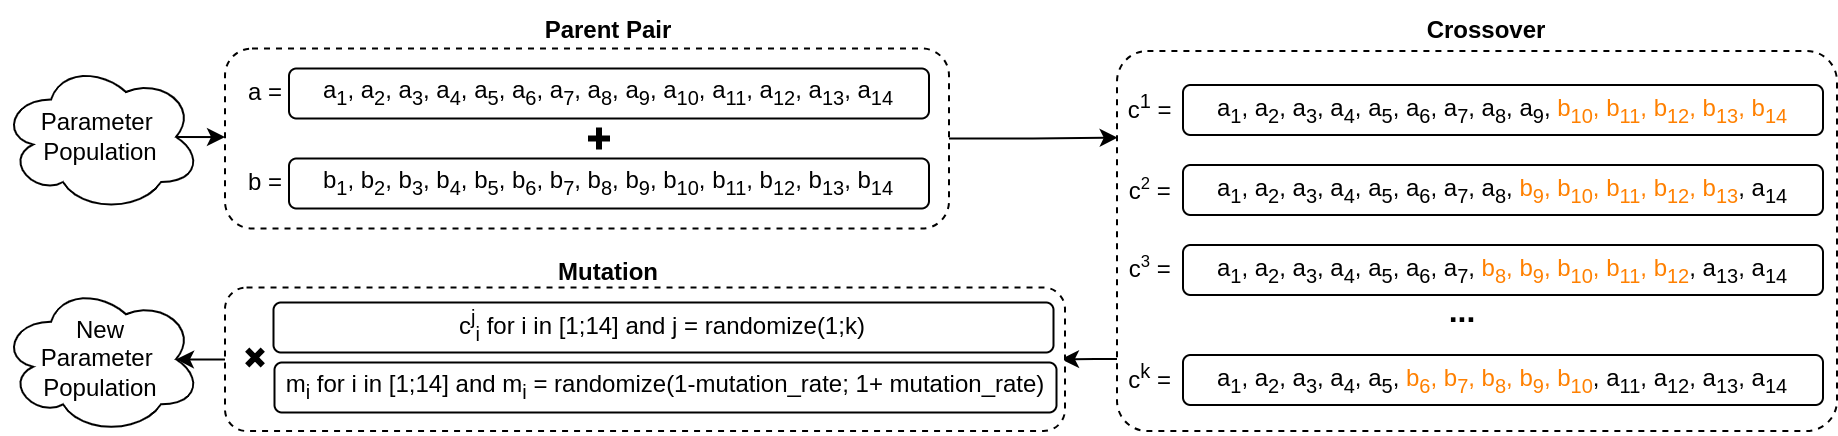
\includegraphics[width=\linewidth]{image/GA2.png}
    \caption{Genetic Algorithm Simulation}
    \label{fig:ga.png}
\end{figure}



%The optimal results were obtained with the following settings: \textit{Population Size} = 100, \textit{Mutation Rate} = 0.1, \textit{Number of Generations} = 100, \textit{n} = 20, and \textit{m} = 5. 
%We evaluated individuals by calculating wallet credit scores from their parameters and converting these scores into credit levels. We then compared these levels to the assigned labels to assess accuracy. The \textit{Fitness Function} was computed using Equation~\ref{accuracy}.

% Để đánh giá cá thể tốt, chúng tôi sử dụng parameters của cá thể đó để tính credit score của các ví trong dataset, từ đó tính ra mức tín dụng rồi so sánh với các nhãn đã gán cho từng ví để đánh giá độ chính xác. Hàm \textit{Fitness Function} được tính theo euquation (3) which assesses the effectiveness of individuals based on the original fuzzy labels of the dataset. Bộ tham số của từng individual sẽ được dùng để tính credit score của các ví trong dataset, từ đó tính ra mức tín dụng rồi so sánh với các nhãn đã gán cho từng ví để đánh giá độ chính xác. The \textit{Fitness Function} used in the genetic algorithm (cf. Equation~\ref{accuracy}) is the accuracy evaluation function of predictions.
\begin{equation}
\label{accuracy}
        accuracy = \frac{\textit{Total number of wallets with correct predicted labels}}{\textit{Total number of wallets predicted}}
\end{equation}

% \begin{equation}
% \label{accuracy}
%     accuracy = \frac{\textit{total predicted labels $y_{pred}$ is the first label $y_{first}$ or the second label $y_{second}$}}{\textit{total predicted labels $y_{pred}$}}
% \end{equation}







%Trong quá trình triển khai, chúng tôi tiến hành fine tune ba tham số chính là Population Size, Mutation Rate, và Number of Generations. Các giá trị fine-tune được thể hiện ở bảng ... Mỗi một lần fine-tune chúng tôi sẽ thực hiện lai tạo đến khi kết quả đạt được thay đổi ít hoặc có dấu hiệu đi xuống. Mỗi một đời chúng tôi sẽ lấy các cá thể dựa trên một tham số Rank Selection cố định là 20 cá thể cho kết quả tốt nhất và 5 cá thể cho kết quả tệ nhất của mỗi đời. Khi lai tạo, Crossover Function được điều chỉnh từ Single-point Crossover sang Two-point Crossover nhằm tăng khả năng tìm kiếm các giải pháp tốt, chấp nhận đánh đổi thời gian huấn luyện lâu hơn.


% \begin{lstlisting}[language=Python,label={accuracy}]
% def CUSTOM_ACCURACY (first_y, second_y, y_pred):
%     condition = numpy.logical_or(y_pred == second_y, y_pred == first_y)
%     count = sum(condition)
%     accuracy = count / len(y_pred)
%     return accuracy 
% \end{lstlisting}
\subsubsection{Stochastic Gradient Descent}
Stochastic Gradient Descent (SGD) is an iterative optimization used to minimize loss functions by updating model parameters. Unlike standard gradient descent, which uses the entire dataset, SGD updates parameters using a single randomly selected training example or a small batch at each iteration, reducing computational costs per iteration. SGD is widely used and performs well across various machine learning tasks \cite{recht2011hogwild}. 

\begin{algorithm}[H]
\caption{Stochastic Gradient Descent Algorithm Implementation}\label{al1}
\label{alg:example}
\begin{algorithmic}[1]
\Require Learning rate $\alpha$, decay rate $decay\_rate$, number of iterations $num\_iterations$
\State Initialize parameter $\theta$
\State Set time step $t = 0$
\For{each iteration $i$ in $num\_iterations$}
    \State Sample a mini-batch of $m$ training examples $x_i$ with corresponding labels $y_{first}^i$, $y_{second}^i$
    \State Compute gradients $g = \frac{1}{m} \nabla_\theta \sum_{i=1}^m J(\theta; x_i, y_{first}^i, y_{second}^i)$
    \State \textbf{Update parameters:} $\theta \leftarrow \theta - \alpha g$
    \State Adjust learning rate: $\alpha \leftarrow \alpha * decay\_rate$
    \State Increment time step: $t \leftarrow t + 1$
\EndFor
\end{algorithmic}
\end{algorithm}

Algorithm~\ref{al1} describes our SGD implementation.
We adapted the loss function to handle multiple labels per wallet (see Table~\ref{tab4}). With the input parameters $y_{first}$ (first label), $y_{second}$ (second label), and $y_{predict}$ (predicted value), the new loss function is defined as shown in Equation~\ref{eq2}.

% In the SGD application section, we adjusted the loss function to fit the problem of assigning 2 labels. With the input parameters, $\mathrm{first\_Y}$ representing the first label, $\mathrm{second\_Y}$ representing the second label, and $\mathrm{Y\_pred}$ representing the predicted value, the new loss function is defined as the formula~\ref{eq2}:

\begin{equation}\label{eq2}
E(i) = \left\{
\begin{array}{ll}
y_{predict}^i - y_{first}^i & \text{if } y_{first}^i = y_{second}^i \\
y_{predict}^i - min(y_{first}^i, y_{second}^i) & \text{if } y_{predict}^i < min(y_{first}^i, y_{second}^i) \\
y_{predict}^i - max(y_{first}^i, y_{second}^i) & \text{if } y_{predict}^i > max(y_{first}^i, y_{second}^i)\\
\end{array}
\right.
\end{equation}

\subsubsection{Adam Algorithm}
The Adam optimizer has gained significant popularity in recent years due to its efficiency and performance~\cite{kingma2014adam}. Unlike traditional SGD algorithms, Adam (Adaptive Moment Estimation) requires fewer resources, converges faster,  and accelerates learning while enhancing overall performance~\cite{yaguchi2018adam}. %Adam combines the advantages of two methods: RMSProp and AdaGrad. 

Adam is a first-order optimization algorithm that can replace traditional stochastic gradient descent. It enhances the optimization process by using first-order moment estimation (momentum) and second-moment estimation (Adadelta). The learning rate for each parameter is dynamically adjusted based on these estimates, and bias correction is applied to stabilize the parameters. The pseudocode in Algorithm~\ref{al2} provides the Adam implementation details. The loss function used in Adam is similar to that in SGD Equation~\ref{eq2})


\begin{algorithm}[H]
\caption{Adam Algorithm Implementation.}\label{al2}
\begin{algorithmic}[1]
\Require Learning rate $\alpha$, number of iterations $num\_iterations$

Exponential decay rates $\beta_1$ and $\beta_2$ for moments $v_t$ and $a_t$ respectively

Small constant $\delta$, for numerical stability
\State Initialize parameter $\theta$, first and second moments $v_t = 0$ and $a_t = 0$.
\State Set time step $t = 0$
\For{each iteration $i$ in $num\_iterations$}
    \State Sample $m$ training examples $x_i$ with corresponding labels $y_{first}^i$, $y_{second}^i$
    \State Compute gradients: $g \leftarrow \frac{1}{m} \nabla_\theta \sum_{i=1}^m J(\theta; x_i, y_{first}^i, y_{second}^i)$
    \State Update time step $t \leftarrow t + 1$
    \State \textbf{First moment:} $v_t = \beta_1 v_{t-1} + (1 - \beta_1) g$
    \State \textbf{Second moment:} $a_t = \beta_2 a_{t-1} + (1 - \beta_2) g \odot g$
    \State \textbf{Bias correction for first moment estimate:} $\hat{v_t} = \frac{v_t}{1 - \beta_1^t}$
    \State \textbf{Bias correction for second moment estimate:} $\hat{a_t} = \frac{a_t}{1 - \beta_2^t}$
    \State \textbf{Compute parameter update:} $\Delta \theta = -\alpha \frac{\hat{v_t}}{\sqrt{\hat{a_t}} + \delta}$
    \State \textbf{Update parameters:} $\theta \leftarrow \theta + \Delta \theta$
\EndFor
\end{algorithmic}
\end{algorithm}


\subsubsection{Multilayer Perceptron}
A Multilayer Perceptron (MLP) is a type of feedforward neural network that uses nonlinear activation functions to model complex patterns in data. It typically comprises three components: an input layer, one or more hidden layers, and an output layer~\cite{8549859}. The input layer receives raw data, which passes through the hidden layers. In each layer, neurons compute a weighted sum of inputs, apply a nonlinear activation function (commonly ReLU), and forward the result to the next layer. The output layer produces the final prediction. 

Figure~\ref{fig:neural_network} illustrates the neural network architecture we designed, consisting of a 14-node input layer (representing wallet features), two hidden layers with 64 and 10 nodes respectively, and a 5-node output layer, corresponding to five credit score levels. %consisting of a 14-node input layer (each node representing a wallet feature), two hidden layers with 64 and 10 nodes respectively, and a 5-node output layer, where each node corresponds to one of the five credit score levels.

In our MLP implementation, we customized the loss function to handle two labels per sample. The input parameters include $y_{first}$ (the first label), $y_{second}$ (the second label), and $y_{predict}$ (the predicted value). The new loss function is defined in Equation~\ref{equa3}, where $ N $ is the number of samples, $ C $ is the number of classes, $ \text{one\_hot}(y_{\text{true}}, c) $ transforms the true label $ y_{\text{true}} $ into a one-hot vector, and $ y_{predict}[i, c] $ represents the predicted probability of class $c$ for sample $i$.



\begin{figure}
    \centering
    \begin{tikzpicture}[node distance=1.5cm]
        \tikzstyle{neuron}=[circle,fill=black!25,minimum size=17pt,inner sep=0pt]
        \tikzstyle{input neuron}=[neuron, fill=black!50];
        \tikzstyle{output neuron}=[neuron, fill=black!50];
        \tikzstyle{hidden neuron}=[neuron, fill=black!50];
        \tikzstyle{annot} = [text width=4em, text centered]
    
        % Input Layer
        \foreach \name / \y in {1,...,5}
            \node[input neuron] (I-\name) at (0,-\y) {};
    
        % Hidden Layer 1
        \foreach \name / \y in {1,...,6}
            \path[yshift=0.5cm]
                node[hidden neuron] (H1-\name) at (2.5,-\y) {};
    
        % Hidden Layer 2
        \foreach \name / \y in {1,...,6}
            \path[yshift=0.5cm]
                node[hidden neuron] (H2-\name) at (5,-\y) {};
    
        % Output Layer
        \foreach \name / \y in {1,...,4}
            \path[yshift=-1cm]
                node[output neuron] (O-\name) at (7.5,-\y) {};
        
        % Connect nodes
        \foreach \source in {1,...,5}
            \foreach \dest in {1,...,6}
                \path (I-\source) edge (H1-\dest);
    
        \foreach \source in {1,...,6}
            \foreach \dest in {1,...,6}
                \path (H1-\source) edge (H2-\dest);
    
        \foreach \source in {1,...,6}
            \foreach \dest in {1,...,4}
                \path (H2-\source) edge (O-\dest);
    
        % Annotate the layers
        \node[annot,below=1cm of H1-5, text width=6em] (hl1){Hidden layer 1 \\ \textbf{(64 nodes)}};
        \node[annot, below=1cm of H2-5, text width=6em](hl2) {Hidden layer 2 \\ \textbf{(10 nodes)}};
        \node[annot, left = 0.5 cm of hl1, text width=6em] {Input layer \\ \textbf{(14 nodes)}};
        \node[annot, right = 0.5 cm of hl2, text width=6em] {Output layer \\ \textbf{(5 nodes)}};
    
    \end{tikzpicture}
    \caption{Neural network architecture}
    \label{fig:neural_network}
\end{figure}






\begin{equation}
\label{equa3}
\begin{gathered}
\text{SCC (Sparse Categorical Crossentropy)} = \sum_{c=1}^{C} \text{one\_hot}(y_{\text{true}}, c) \cdot \log(y_{predict}[c])
\\
\text{Loss} = -\frac{1}{N} \sum_{i=1}^{N} \min(\text{SCC}(y_{first}[i], y_{predict}[i]), \text{SCC}(y_{second}[i], y_{predict}[i]))
\end{gathered}
\end{equation}

% Where:
% \begin{itemize}
%     \item $ N $ is the number of samples
%     \item $ C $ is the number of classes
%     \item $ \text{one\_hot}(y_{\text{true}}, c) $: transforms the true label $ y_{\text{true}} $ into a one-hot vector
%     \item $ y_{\text{pred}}[i, c] $ represents the predicted probability of class $c$ for sample $i$
% \end{itemize}


% \begin{algorithm}
% \caption{Crossover Methods}
% \begin{algorithmic}[1]

% \Function{custom\_accuracy}{first\_y, second\_y, y\_pred}
%     \State condition $\gets$ \text{np.logical\_or}(y\_pred == \text{second\_y}, y\_pred == \text{first\_y})
%     \State count $\gets$ \text{sum}(condition)
%     \State accuracy $\gets$ count / \text{len}(y\_pred)
%     \State \Return accuracy
% \EndFunction


% \end{algorithmic}
% \end{algorithm}
% \subsubsection{MLP}

\section{EXPERIMENT}\label{section4}
% The dataset was split into two parts: (1) a training set for model development and (2) a testing set for evaluation.
% We assess the performance of the methods using \textbf{Accuracy} and \textbf{Precision} metrics. Given that some predictions may correspond to multiple correct labels (refer to Table~\ref{tab4}), \textbf{Recall} (detection rate) could not be computed and was excluded from the evaluation. The experimental results are summarized in Table~\ref{tab:results}.

% We evaluated the performance of the proposed methods using \textbf{Accuracy}, \textbf{Precision}, and \textbf{Recall} metrics. The results are summarized in Table~\ref{tab:results}. %Since some predictions correspond to multiple correct labels (as shown in Table~\ref{tab4}), \textbf{Recall} was excluded from the evaluation due to its inapplicability.




\begin{comment}
Before applying any method, the original dataset was divided into two parts: (1) the training dataset and (2) the testing dataset. The training dataset is used to train the model, while the testing dataset is used to evaluate the accuracy of the model. This ensures that the model not only memorizes the data it has seen but also has good generalization ability on new data. Typically, the dataset is split in an 80:20 ratio, with 80\% for training and 20\% for testing. However, this ratio may vary depending on the specific problem and can be adjusted to achieve the best results.

In this section, the results of the methods are presented and evaluated using two main performance metrics:

\textbf{Accuracy:} Accuracy is the most widely used classification performance metric. It calculates the number of correctly classified samples by the model out of the total samples in the dataset. Accuracy is calculated as explained in Equation.~\ref{eq3}

\begin{equation}\label{eq3}
    \text{Accuracy} = \frac{\text{Count of Correct Predictions}}{\text{Total Number of Predictions}}
\end{equation}

\textbf{Precision:} Precision is a metric used to evaluate the accuracy of correctly classified positive samples by the model. It is calculated by dividing the number of TP by the sum of TP and FP. In simpler terms, precision measures how many of the classified TP instances are actually positive. Precision is calculated as explained in Equation~\ref{eq4}

\begin{equation}\label{eq4}
    \text{Precision} = \frac{\text{TP}}{\text{TP} + \text{FP}}
\end{equation}

In some cases, each prediction may have more than one correct label. For instance, a wallet, which has a borrow-to-asset ratio over 40\% and more than one liquidation, can be Poor or Fair. As a result, Recall (Detection Rate) cannot be calculated. Therefore, Recall should not be used to evaluate the performance of the models in this case.
\end{comment}

\textbf{SGD and Adam: }
% \subsubsection{SGD, Adam}
% \paragraph{}
We implemented Stochastic Gradient Descent (SGD) and Adam optimizers, tuning both the learning rate and number of iterations. For SGD, we set a decay rate of 0.95. The Adam optimizer was configured with the parameters $\beta_1 = 0.9$; $\beta_2 = 0.999$; and $\epsilon = 1\times10^{-8}$ . We tested learning rates of 0.1, 0.01, and 0.001 across 100, 1000, and 10 000 iterations. The best results for both algorithms were achieved with a learning rate of 0.001 and 10 000 iterations.
% After determining the evaluation method, we proceeded to implement the models. For SGD, we initialized the $decay\ rate = 0.95$. The corresponding parameters for Adam include $\beta_1 = 0.9$, $\beta_2 = 0.999$, and $\epsilon = 1\times10^{-8}$. Both algorithms were tested with different values of learning rate and number of iterations. Specifically, the learning rates included values of $0.1$, $0.01$, and $0.001$, and the number of iterations included values of $100$, $1000$, and $10000$. After implementation, both SGD and Adam algorithms yielded the best results at a learning rate of $0.001$ and number of iterations of $10000$.

%Sau khi xác định được phương pháp đánh giá, chúng tôi tiến hành triển khai các models. Đối với SGD, chúng tôi khởi tạo than số  decay rate là 0.95. Các tham số  tương ứng đối với Adam bao gồm beta1 là 0.9, beta2 là 0.999, và epsilon là 1e-8. Cả hai thuật toán đều được thử nghiệm với các giá trị learning rate và number iterations khác nhau. Cụ thể, learning rate bao gồm  các giá trị là 0.1, 0.01, 0.001, và number iterations bao gồm  các giá trị 100, 1000, 10000. Sau khi triển khai, cả 2 thuật toán SGD, Adam cho kết quả tốt nhất tại learning rate là 0.001 và number iterations là 10000.

\textbf{Genetic Algorithm: }
% \subsubsection{Genetic Algorithm}
% \paragraph{}
For GA, we initialized the number of generations to 100 and experimented with various crossover functions and mutation rates. The two-point crossover and a mutation rate of 0.1 produced the best results after testing one-point and two-point crossovers and mutation rates of 0.1 and 0.2.
% For the GA algorithm, we initialized the number of generations parameter to $100$. From this parameter, we tested the model with different crossover functions and different mutation rates. Mutation rates of $0.1$ and $0.2$, and crossover functions of one-point and two-point were used. After implementation and evaluation, the two-point crossover function combined with a mutation rate of $0.1$ gives the best results.

%Đối với giải thuât GA, chúng tôi khởi tạo tham số number generations là 100. Từ tham số này, chúng tôi thử nghiệm mô hình với các hàm lai tạo khác nhau với các tỉ lệ đột biến khác nhau. Tỉ lệ đột biến 0.1, 0.2, và hàm lai tạo one point, two point được chúng tôi sử dụng. Sau khi triển khai và đánh giá thì hàm lai tạo two point kêt hợp với tỉ lệ đột biến 0.1 cho kết quả tốt nhất.
\textbf{Multilayer Perception: }
% \subsubsection{Multilayer Perception}
% \paragraph{}
We experimented with multiple neural network architectures, the number of epochs, and batch sizes. The best performance was achieved with two hidden layers (see Figure~\ref{fig:neural_network}), 10 epochs, and a batch size of 64.
% For Multilayer Perceptron, we tested the model with different neural network architectures, as well as varying the number of epochs and batch sizes. Specifically, the values for epochs included 5, 10, and 20, while the values for batch size included 32 and 64. After implementation, the model with 2 hidden layers, as introduced above, along with 10 epochs and a batch size of 64, gives the best results.


%Bảng đưa ra kết quả trên tập test khi triển khai bốn mô hình. Kết quả bao gồm bốn chỉ số accuracy, precision và recall từ tổng quan đến chi tiết từng labels: poor, fair, good, very good và excellent. Từ kết quả này chúng tối rút ra được ba kết luận như sau.
Table~\ref{tab:results} and Figure~\ref{fig:model_comparison} present and compare the performance of the four models on the test dataset, covering three metrics: accuracy (A), precision (P), and recall (R), for each separated label and for all labels. The key findings are as follows: %present and compare the performance results on the test dataset after implementing four models. The results encompass three metrics: accuracy (A), precision (P), and recall (R), provided both overall and in detail for each label: \textit{Poor}, \textit{Fair}, \textit{Good}, \textit{Very Good}, and \textit{Excellent}. Based on these outcomes, we draw the following key conclusions:


(1) The MLP model achieved the highest performance, with 97.93\% accuracy and 90.68\% precision. In comparison, the GA model had slightly lower performance, with 97.5\% accuracy and 90.30\% precision, but surpassed the MLP in recall (62\% vs. 58.96\%). The SGD model exhibited the lowest performance, with 64.03\% accuracy and 53\% precision.

%(1) MLP cho kết quả tốt nhất với ACC ... và precision ... So với MLP, GA cũng đạt kết quả chỉ thấp hơn một chút với Acc và precison .. thậm chí recall của ga () cao hơn so với mlp (). SGD cho kết quả tồi nhất khi chi có ... ACC và ... precision.
% (1) The MLP model achieves the best performance, with an accuracy of 97.93\% and a precision of 90.68\%. In comparison, the GA model also produces slightly lower results with an accuracy of 97.5\% and a precision of 90.30\%. Moreover, the recall of the GA model (62\%) surpasses that of the MLP (58.96\%). On the other hand, the SGD model exhibits the poorest performance, with an accuracy of 64.03\% and a precision of 53\%.


%(2) Hai nhãn Fair và Good là hai nhãn có kết quả dự đoán tốt nhất. Cụ thể , với nhãn Fair kết quả (accuracy, precision, recall) trên lần lượt hai mô hình GA và MLP là (97.65; 99.05; 97.86) và (98.66; 97.09; 98.91). Kết quả GA và MLP với nhãn Good là (94.43; 94.50; 75.54) và (98.27; 97.09; 91.77). Điều này được thể hiện rõ ràng hơn tại Figure 3, khi mô hình MLP dữ đoán đúng chính xác các ví chắc chắn là Fair và Good.
(2) The \textit{Fair} and \textit{Good} labels had the most accurate predictions. For the \textit{Fair} label, the results (A, P, R) for the GA and MLP models are (97.65\%; 99.05\%; 97.86\%) and (98.66\%; 97.09\%; 98.91\%), respectively. For the \textit{Good} label, GA and MLP results are (94.43\%; 94.50\%; 75.54\%) and (98.27\%; 97.09\%; 91.77\%), respectively. Figure~\ref{fig:heatmap} further illustrates that the MLP model accurately predicted instances with high confidence in the \textit{Fair} and \textit{Good} labels.





%(3) Kết quả recall của các mô hình thấp tại một số nhãn. Đối với MLP, giá trị recall thấp tại hai nhãn Poor và Excellent với lần lượt là 7.4% và 24.10%. Trong khi đó, GA có recall thấp tại hai nhãn Poor và Very Good với lần lượt là 22.90% và 15.05%. Điều này gây ra bởi việc đầu vào nhãn dữ liệu là fuzzy labeling trong khi đầu ra của mô hình chỉ là một trong năm nhãn Fair, Good, Very Good và Excellent. Cụ thể , tập ví được gán các nhãn (Poor, Poor), (Poor, Fair), (Fair, Fair) khi được model dự đoán chủ yếu có nhãn là Fair dẫn đến giá trị recall của nhãn Fair cao còn nhãn Poor sẽ thấp.
(3) Recall values were notably low for certain labels across the models. For the MLP model, recall is particularly low for the \textit{Poor} and \textit{Excellent} labels, at 7.4\% and 24.10\%, respectively. The GA model also shows low recall for the \textit{Poor} and \textit{Very Good} labels, with values of 22.90\% and 15.05\%, respectively. This discrepancy arises from the use of fuzzy labeling in the test dataset, while the model outputs are a selection among the five labels: \textit{Fair}, \textit{Good}, \textit{Very Good}, and \textit{Excellent}. Specifically, samples labeled as (\textit{Poor, Poor}), (\textit{Poor, Fair}), and (\textit{Fair, Fair}) were predominantly predicted as \textit{Fair}, resulting in high recall for the \textit{Fair} label but low recall for the \textit{Poor} label.


% \begin{table}[h!]
% \centering
% \caption{The performance of the optimized models}
% \label{tab:results}
% \begin{tabularx}{\textwidth}{|Y|l|Y|Y|c|c|}
% \hline
% \multicolumn{2}{|c|}{\textbf{Model}}& SGD &  Adam  & Genetic Algorithm & Multilayer Perception\\          
% \hline
% \multicolumn{2}{|c|}{\textbf{Accuracy} (\%)} & 76.56 & 95.12 & 96.94 & 97.50\\
% \hline
% \multirow{6}{*}{\rotatebox{90}{\textbf{Precision} (\%)}}
% & \textbf{Overall} & 35.11 & 82.50  & 85.78 &  91.65\\
% \cline{2-6}
% &\textbf{Poor}& 14.67        & 64.20         & 83.61            & 90.91     \\
% \cline{2-6} 
% &\textbf{Fair} & 97.44        & 96.72         & 99.34            & 97.80     \\
% \cline{2-6} 
% &\textbf{Good} & 68.14        & 72.56         & 93.06            & 98.29     \\
% \cline{2-6} 
% &\textbf{Very Good} & 4.09         & 40.44         & 53.37            & 72.66     \\
% \cline{2-6} 
% &\textbf{Excellent} & 26.37        & 53.57         & 76.47            & 100.00    \\
% \hline
% \end{tabularx}
% \end{table}

% \begin{table}[h!]
% \centering
% \caption{The performance of the optimized models}
% \label{tab:results}
% \begin{threeparttable}
% \footnotesize
% \begin{tabularx}{\textwidth}{|Y|c|c|c|c|c|c|c|c|c|c|c|c|}
% \hline
% \multirow{2}{*}{\textbf{Model}} & \multicolumn{3}{c|}{\textbf{SGD}} &  \multicolumn{3}{c|}{\textbf{Adam}}  & \multicolumn{3}{c|}{\textbf{GA}} & \multicolumn{3}{c|}{\textbf{MLP}}\\          
% \cline{2-13}
%  & \textit{A} & \textit{P} & \textit{R} & \textit{A} & \textit{P} & \textit{R} & \textit{A} & \textit{P} & \textit{R} & \textit{A} & \textit{P} & \textit{R}\\
% \hline
% \textbf{Overall} & 64.03 & 53.00 & 40.60 & 96.1 & 81.83 & 51.10 & 97.50 & 90.30 & 62.0 & 97.93 & 90.68 & 58.96 \\
% \hline
% \textbf{Poor} & 57.30 & 0.95 & 35.75 & 98.73 & 43.27 & 41.34 & 99.05 & 77.36 & 22.90 & 96.88 & 85.07 & 7.40 \\
% \hline
% \textbf{Fair} & 53.67 & 96.20 & 40.90 & 95.93 & 97.99 & 96.65 & 97.65 & 99.05 & 97.86 & 98.66 & 97.09 & 98.91\\
% \hline
% \textbf{Good} & 80.00 & 14.30 & 47.16 & 93.94 & 92.72 & 75.1 & 94.43 & 94.50 & 75.54 & 98.27 & 97.09 & 91.77\\
% \hline
% \textbf{Very Good} & 79.50 & 11.90 & 94.60 & 83.03 & 93.85 & 28.23 & 79.97 & 88.62 & 15.05 & 98.57 & 86.24 & 72.55 \\
% \hline
% \textbf{Excellent} & 88.00 & 100.00 & 26.00 & 96.20 & 81.36 & 14.14 & 99.57 & 91.78 & 98.67 & 98.35 & 86.36 & 24.10 \\
% \hline
% \end{tabularx}
% \begin{tablenotes}
%       \small
%       \item \textit{A}: Accuracy (\%), \textit{P}: Precision (\%), \textit{R}: Recall (\%)
% \end{tablenotes}
% \end{threeparttable}
% \end{table}

\begin{table}[h!]
\centering
\caption{The performance of the optimized models}
\label{tab:results}
\begin{threeparttable}
\footnotesize
\begin{tabularx}{\textwidth}{|Y|c|c|c|c|c|c|c|c|c|c|c|c|}
\hline
\multirow{2}{*}{\textbf{Label}} & \multicolumn{4}{c|}{\textbf{Accuracy} (\%)} &  \multicolumn{4}{c|}{\textbf{Precision} (\%)}  & \multicolumn{4}{c|}{\textbf{Recall} (\%)}\\          
\cline{2-13}
 & \textit{SGD} & \textit{Adam} & \textit{GA} & \textit{MLP} & \textit{SGD} & \textit{Adam} & \textit{GA} & \textit{MLP} & \textit{SGD} & \textit{Adam} & \textit{GA} & \textit{MLP}\\
\hline
\textbf{Overall} & 64.03 & 96.10 & 97.50 & 97.93 & 53.00 & 81.83 & 90.30 & 90.68 & 40.60 & 51.10  & 62.0 & 58.96 \\
\hline
\textbf{Poor} & 57.30 & 98.73 & 99.05 & 96.88 & 0.95 & 43.27 & 77.36 & 85.07 & 35.75  & 41.34  & 22.90 & 7.40 \\
\hline
\textbf{Fair} & 53.67 & 95.93 & 97.65 & 98.66 & 96.20 & 97.99 & 99.05 & 98.66 & 40.90 & 96.65 & 97.86 & 98.91\\
\hline
\textbf{Good} & 80.00 & 93.94 & 94.43 & 98.27 & 14.30 & 92.72 & 94.50 & 97.09 & 47.16 & 75.1 & 75.54 & 91.77\\
\hline
\textbf{Very Good} & 79.50 & 83.03 & 79.97 & 98.57 & 11.90 & 93.85 & 88.62 & 86.24 & 94.60 & 28.23 & 15.05 & 72.55 \\
\hline
\textbf{Excellent} & 88.00 & 96.20 & 99.57 & 98.35 & 100.00 & 81.36 & 91.78 & 86.36 & 26.00 & 14.14 & 98.67 & 24.10 \\
\hline
\end{tabularx}
% \begin{tablenotes}
%       \small
%       \item \textit{A}: Accuracy (\%), \textit{P}: Precision (\%), \textit{R}: Recall (\%)
% \end{tablenotes}
\end{threeparttable}
\end{table}

\begin{figure}[h!]
    \centering
    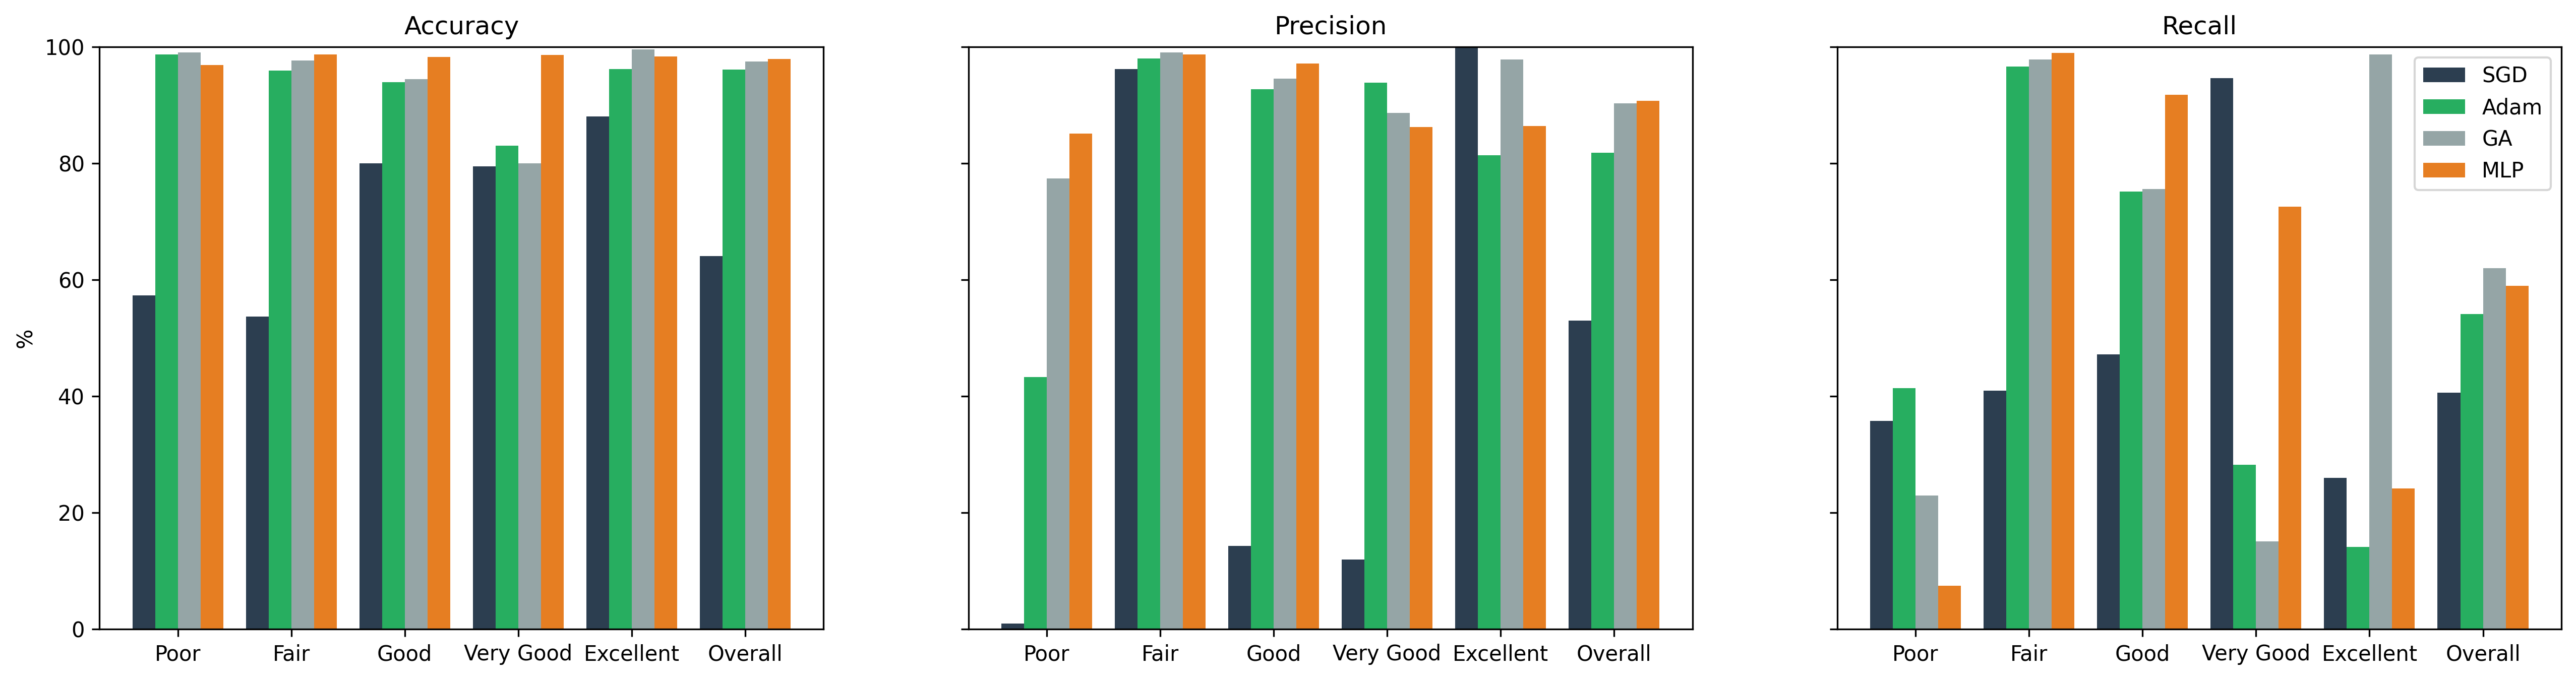
\includegraphics[width=\textwidth]{image/model_comparison.png}
    \caption{Model Comparison}
    \label{fig:model_comparison}
\end{figure}

Figure \ref{fig:heatmap} provides a heatmap visualizing the MLP's predictions compared to the original fuzzy labels. In the heatmap, the Y-axis represents the predicted credit levels: 0 (Poor), 1 (Fair), 2 (Good), 3 (Very Good), and 4 (Excellent). The X-axis corresponds to the fuzzy labels assigned to the test dataset. Using the Fuzzy Labeling approach, each wallet address is assigned two labels, reflecting the uncertainty in classification. For example, a label of (0;0) indicates a definitive classification of \textit{Poor}, while a label of (0;1) suggests that the wallet could be classified as either \textit{Poor} or \textit{Fair}. Thus, the test dataset contains these fuzzy label pairs, such as (0;0), (0;1), (1;2), and (4;4).


Each cell in the heatmap shows the number of wallets predicted at a specific level, compared to their original fuzzy labels. For example, a cell displaying 644 indicates that 644 wallets were predicted to be at level 1 (Fair), while their original fuzzy labels were (0, 1), meaning they could belong to either Poor or Fair.

\begin{figure}[h!]
    \centering
    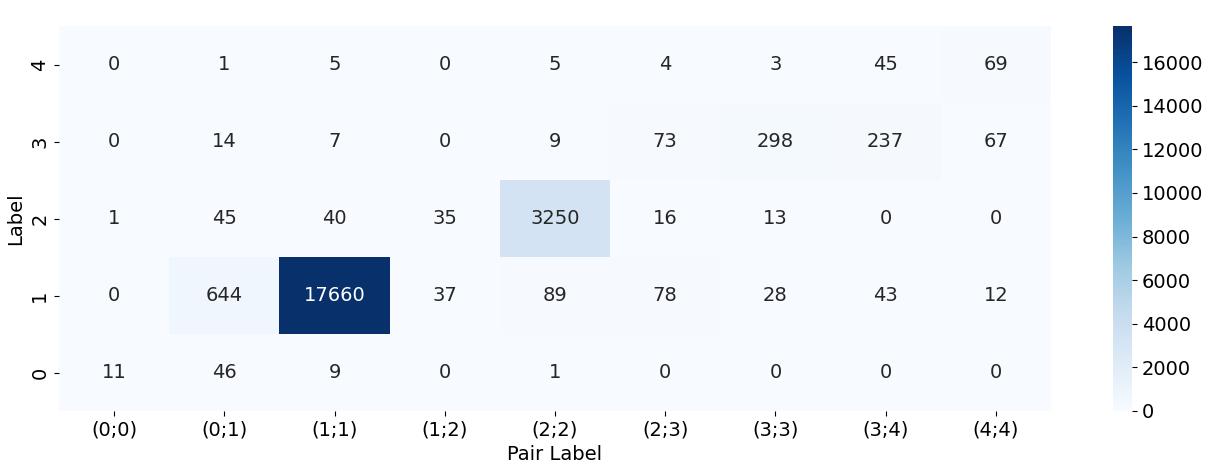
\includegraphics[width=\textwidth]{image/heatmap.png}
    \caption{Heatmap of Predicted Credit Levels and Fuzzy Labels}
    \label{fig:heatmap}
\end{figure}

\section{CONCLUSION}\label{section5}
This study applied optimization techniques including Stochastic Gradient Descent (SGD), Adam Optimization Algorithm, Genetic Algorithm (GA), and Multilayer Perceptron (MLP) to optimize the credit scoring formula for crypto wallets on the DeFi platform.
% To address the challenges of determining precise credit levels, a fuzzy labeling approach was applied, allowing each wallet to receive multiple possible credit levels. 
While SGD, Adam, and MLP models classified wallet credit into five levels, the Genetic Algorithm provided detailed credit scores ranging from 300 to 850. Among these techniques, the Multilayer Perceptron achieved the highest performance, with an accuracy of 97.93\% and a precision of 90.68\%.
These results highlight the potential of advanced algorithms and machine learning models to improve credit scoring systems in DeFi. The use of fuzzy labeling helps manage uncertainty in credit classification, leading to more accurate risk assessments and greater transparency in lending practices. This contributes to the development of more reliable and transparent financial practices.

Future research should expand the dataset to include non-EVM chains like Cosmos\footnote{\href{https://cosmos.network/}{https://cosmos.network}}, Solana\footnote{\href{https://solana.com/}{https://solana.com}}, and Polkadot\footnote{\href{https://polkadot.network/}{https://polkadot.network}} to test the models in diverse blockchain environments. Additionally, an automated labeling system will further enhance scoring accuracy and streamline evaluation, promoting the integration of robust credit scoring mechanisms in decentralized finance.



% Experimental results showed that the Multilayer Perceptron achieved the highest efficiency compared to the other techniques.
% Trong khi 3 mô hình SGD, Adam, và MLP chỉ xếp hạng được tín dụng ví theo 5 mức, GA lại có thể tính được điểm tín dụng cụ thể từ 300-850.
% However, since the main objective of the study is to determine the optimal parameter set for the credit scoring formula, the Genetic Algorithm is considered a more suitable choice. The reasons for this choice are as follows:

% \begin{itemize} \item Genetic Algorithm provides higher interpretability compared to Multilayer Perceptron, making it easier for users to understand the basis for the scoring results. \item Genetic Algorithm can produce a specific score compared to MLP, which only provides score ranges. \item Genetic Algorithm can integrate conditions for the parameters, allowing conditions to be changed clearly.  \end{itemize}

% The study also indicates that using public blockchain data can significantly benefit optimizing machine learning models. This data provides a rich source of information and easy access to build and evaluate models, enhancing the efficiency and transparency of decentralized financial systems. In the future, we will expand this data from None-EVM chains like Cosmos~\footnote{\href{https://cosmos.network/}{https://cosmos.network}}, Solana~\footnote{\href{https://solana.com/}{https://solana.com}}, Polkadot~\footnote{\href{https://polkadot.network/}{https://polkadot.network}}, etc. We also focus on establishing an efficient mechanism for labeling this data. Based on labeled data, we do a backtest for optimizing models to demonstrate that our score can be applied in real life.

\vspace{2mm}

\subsubsection*{Acknowledgements} This research was supported by~\href{https://centic.io/}{Centic.io}. We would like to show our gratitude to them for sharing their pearls of wisdom with us during this research.


%
% ---- Bibliography ----
%
% BibTeX users should specify bibliography style 'splncs04'.
% References will then be sorted and formatted in the correct style.
%

% \bibliography{mybibliography}
%
% \begin{thebibliography}{99}
% \footnotesize
% \itemsep=-3pt plus.2pt minus.2pt
% \baselineskip=13pt plus.2pt minus.2pt

\bibliographystyle{splncs04nat}
\bibliography{sample-base}

% \bibitem{1}Sayah J Y, Kime C R. Test scheduling in high performance VLSI system implementations. {\it IEEE Trans. Computers}, 1992, 41(1): 52-67. [\textcolor{blue}{example for journal paper}]

% \bibitem{2} Gordon Plotkin. A semantics for type checking. In {\it Lecture Notes in Computer Science 526,} Ito T, Meyer A R (eds.), Springer-Verlag, 1991, pp.1-17. [\textcolor{blue}{example for book chapter}]

% \bibitem{3} Geddes K O, Czapor S R, Labahn G. Algorithms for Computer Algebra. Boston: Kluwer, 1992. [\textcolor{blue}{example for book}]

% \bibitem{4} Kwan A W, Bic L. Distributed memory computers. In {\it Proc. the 6th Int. Parallel Processing Symp.}, March 1992, pp.10-17. [\textcolor{blue}{example for conference}]

% \bibitem{5} Harris M J. Real-time cloud simulation and rendering [Ph.D. Thesis]. Department of Computer Science, The University of North Carolina at Chapel Hill, 2003. [\textcolor{blue}{example for thesis}]

% \bibitem{6} Jurczyk M, Coldwind G. Identifying and ex-ploiting windows kernel race conditions via mem-ory access patterns. Technical Report, Google Re-search, 2013. http://pdfs.semanticscholar.org/ca60/2e7193f159a56a3559-f08b677abfba60beb2.pdf, Mar. 2018. [\textcolor{blue}{example for technical report}]

% \bibitem{7} Gipp B, Meuschke N, Gernandt A. Decentra-lized trusted timestamping using the crypto cur-rency Bitcoin. arXiv:1502.04015, 2015. https://arxiv.org/abs/1502.04015, May. 2018. [\textcolor{blue}{example for ar-Xiv document}]

% \bibitem{8} Tong Y, Chen L, Zhou Z, JagadishH V, Shou L, Lv W. SLADE: A smart large-scale task decomposer in crowdsourcing. {\it IEEE Transactions on Knowledge and Data Engineering}. doi:10.1109/TKDE.2018.2797962. (preprint) [\textcolor{blue}{example for preprint}]

% \end{thebibliography}
\end{document}
